%  LaTeX support: latex@mdpi.com 
%  MDPI Remote Sensing template (ACS citation style)

\documentclass[remotesensing,article,submit,moreauthors]{Definitions/mdpi} 

%=================================================================
% MDPI internal commands - do not modify
\firstpage{1} 
\makeatletter 
\setcounter{page}{\@firstpage} 
\makeatother
\pubvolume{1}
\issuenum{1}
\articlenumber{0}
\pubyear{2026}
\copyrightyear{2026}
\datereceived{ } 
\daterevised{ } 
\dateaccepted{ } 
\datepublished{ } 

%=================================================================
% Full title of the paper
\Title{A Lightweight Convolutional Neural Network-Based Method for Extremely Low-Light RAW Image Enhancement}

% Authors
\Author{Xin Zhao $^{1}$ and Sihai You $^{1,*}$}

\AuthorNames{Xin Zhao and Sihai You}

% Affiliations / Addresses
\address{%
$^{1}$ \quad Rocket Force University of Engineering, Xi'an, China;
xinzh865@buaa.edu.cn (X.Z.); yousihai12345@163.com (S.Y.)}

% Contact information of the corresponding author
\corres{Correspondence: yousihai12345@163.com}

% Abstract
\abstract{Extremely low-light RAW image enhancement is critical for applications such as surveillance and night photography, yet existing methods mostly rely on large-parameter diffusion models or deep Transformers, which incur high computational cost and are difficult to deploy in real time. Targeting efficiency, this paper proposes a lightweight fully-convolutional U-Net that takes white-balanced packed Bayer RAW as input and jointly performs denoising and brightness recovery in a single forward pass. We adopt the dev-RAW evaluation protocol, which uses a long-exposure RAW developed by a fixed ISP as the supervisory reference, avoiding JPG--RAW misalignment and ISP inconsistency. Instead of training a separate model for each illuminance level, a single model covers the three illuminance levels of the SIED dataset (0.01--0.1 / 0.001--0.01 / 0.0001--0.001~lx) without any illuminance prior. On the official SIED Sony 0.01--0.1~lx test set (180 scenes, dev-RAW protocol), the proposed method (base\_ch$=$32, with SE) achieves 34.37~dB PSNR / 0.9059 SSIM, 13.31~dB higher than the fixed-ISP gain baseline (21.06~dB) and significantly better than a SID-style learning baseline trained under the same setting (16.78~dB, due to the JPG-target supervision-domain mismatch). This configuration has only 7.82M parameters and runs at 17.8~FPS on a V100; compressed to base\_ch$=$8 it has only 0.49M parameters at 82.6~FPS; on the edge device Jetson Orin Nano Super, base\_ch$=$8 reaches 5.98/7.61~FPS in fp32/fp16. The single model generalizes across cameras without fine-tuning (Canon: 33.05~dB), and its PSNR drops gracefully from 34.37~dB to 31.74~dB across the three illuminance levels. The results show that lightweight CNNs can deliver usable quality at minimal cost for extremely low-light RAW enhancement, providing a practical solution for resource-constrained scenarios.}

% Keywords
\keyword{low-light image enhancement; RAW image processing; lightweight network; U-Net; channel attention; dev-RAW protocol} 

%=================================================================
% Layout adjustment: use symmetric margins so the body text is centered
% (the default MDPI layout reserves a 5.86cm left margin-par column that
%  is only populated on the first page, leaving large blank space on
%  subsequent pages).
\geometry{left=1.27cm, right=1.27cm, marginparwidth=0cm, marginparsep=0cm}
\setlength{\extralength}{0pt}
\renewcommand{\contentleftcolumn}{}
\fancyheadoffset[L]{0pt}
\fancyfootoffset[L]{0pt}

\begin{document}

%%%%%%%%%%%%%%%%%%%%%%%%%%%%%%%%%%%%%%%%%%
\section{Introduction}

\begin{figure}[H]
\centering
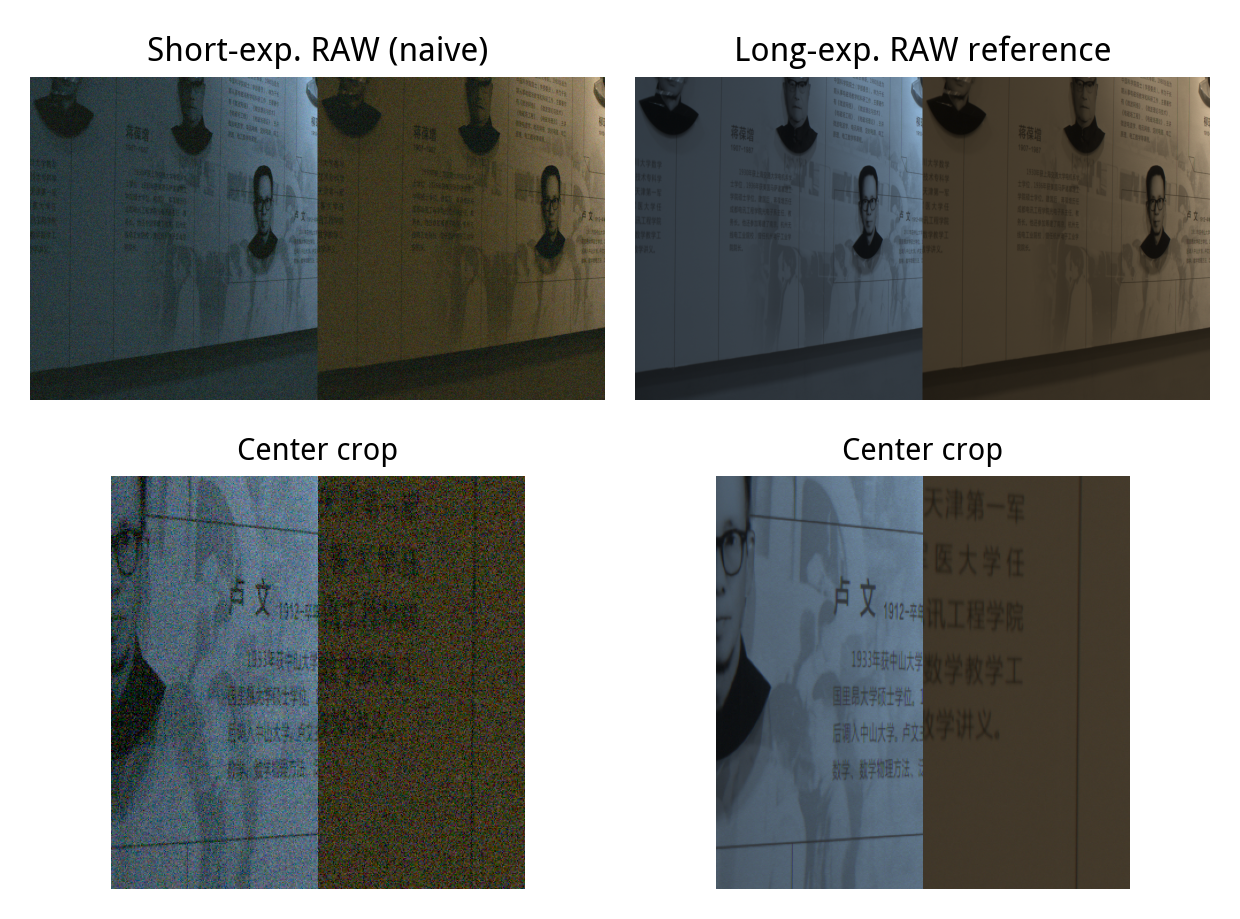
\includegraphics[width=\linewidth]{figures/fig1_motivation.png}
\caption{Motivation. Left column: an extremely low-light short-exposure RAW directly amplified by a fixed ISP (severe noise and color cast). Right column: the long-exposure RAW reference (clear). Top/bottom rows show the full frame and a center crop. The gap highlights the challenge of extremely low-light RAW enhancement.}
\label{fig:motivation}
\end{figure}

In applications such as night photography, surveillance, and astronomical imaging, the ambient light is extremely weak. Short exposures collect scarce photons, leaving the RAW data noise-dominated; direct amplification therefore yields severe noise and color casts. As shown in Figure~\ref{fig:motivation}, the short-exposure RAW directly amplified by a fixed ISP suffers from severe noise and color casts and has a large gap with the long-exposure reference, intuitively illustrating the challenge---traditional ISP amplification alone is far from sufficient to produce a usable image. Traditional methods such as LIME~\citep{guo2017lime} and RetinexNet~\citep{wei2018retinexnet} mostly operate in the sRGB domain and cannot exploit the linear physical characteristics of the RAW domain. Chen \emph{et al.} proposed SID~\citep{chen2018sid}, the first end-to-end learned enhancement in the RAW domain, which significantly outperformed sRGB-domain methods. In recent years, however, quality-oriented methods have trended toward heavier models: diffusion models (SIED~\citep{jiang2025sied}, LDM-ISP~\citep{wen2023ldmisp}, LightenDiffusion~\citep{jiang2024lightendiffusion}), Mamba architectures (Retinex-RAWMamba~\citep{chen2024rawmamba}, HiMA~\citep{chen2025hima}), and Transformers (Restormer~\citep{zamir2022restormer}, Retinexformer~\citep{cai2023retinexformer}) improve restoration quality but at the cost of sharply increased parameters and latency. SIED~\citep{jiang2025sied} requires prolonged two-stage optimization and iterative sampling at inference, making it difficult to deploy on resource-constrained platforms. Recent efficiency-oriented methods such as FLOL~\citep{benito2025flol} and DarkIR~\citep{feijoo2025darkir} mostly operate in the sRGB domain and do not fully exploit the linear RAW signal.

The core question of this paper is: to what extent can the network be compressed while maintaining acceptable restoration quality? We design a family of U-Nets with adjustable channel widths (base\_ch$=$8/16/32) and systematically evaluate their quality--efficiency trade-off under the dev-RAW protocol. The contributions are as follows:

\begin{enumerate}
\item \textbf{dev-RAW evaluation protocol.} Using a long-exposure RAW developed by a fixed ISP as the reference avoids JPG--RAW misalignment and ISP inconsistency, placing the supervision signal and the input in the same signal domain.
\item \textbf{Single-model multi-illuminance coverage.} Unlike SIED~\citep{jiang2025sied}, which trains a separate model for each of the 0.01--0.1 / 0.001--0.01 / 0.0001--0.001~lx levels, we train a \textbf{single model on the combined data of all three SIED illuminance levels (5040 paired synthetic samples)}, without any illuminance prior.
\item \textbf{Lightweight architecture.} The base\_ch$=$32 U-Net has only 7.82M parameters and reaches 17.8~FPS on a V100; base\_ch$=$8 has only 0.49M parameters at 82.6~FPS, making it one of the lightest extremely low-light RAW enhancement models known, and its real-time capability is verified on a Jetson edge device (base\_ch$=$8 reaches 5.98/7.61~FPS at fp32/fp16). The SE channel attention brings a +0.46~dB gain with less than 1\% parameter overhead.
\item \textbf{Honest evaluation-baseline statement.} We explicitly distinguish the dev-RAW reference from the sRGB/JPG reference, do not directly compare numbers with SIED and other methods, and emphasize that this work is efficiency-oriented rather than quality-oriented.
\end{enumerate}

Section~\ref{sec:related} surveys related work, Section~\ref{sec:method} details the proposed method and experimental settings, Section~\ref{sec:results} reports the results and ablations, and Sections~\ref{sec:discussion} and~\ref{sec:conclusion} provide a discussion and concluding remarks.

%%%%%%%%%%%%%%%%%%%%%%%%%%%%%%%%%%%%%%%%%%
\section{Related Work}
\label{sec:related}

\subsection{Low-Light Image Enhancement}

Low-light image enhancement methods fall into non-learning and learning families. The former rely on hand-crafted priors---LIME~\citep{guo2017lime} refines an illumination map under Retinex theory, and histogram-based approaches boost contrast by re-distributing intensity levels---and are lightweight and interpretable, but cannot model the signal-dependent noise that dominates under extremely low light; here they serve only as lightweight post-processing baselines (Table~\ref{tab:main}). Learning approaches can be grouped by architecture. Early Retinex-network families factor the input into reflectance and illumination terms and restore each branch independently (RetinexNet~\citep{wei2018retinexnet}, KinD~\citep{zhang2019kind}); later unrolled variants embed the physical model into deep iterations (URetinex-Net~\citep{wu2022uretex}), and zero-reference curve estimation removes the need for paired supervision (Zero-DCE~\citep{guo2020zerodce}). Other paradigms include SNR-driven design (SNR-Aware~\citep{xu2022snraware}), normalizing-flow illumination modeling (LLFlow~\citep{wang2022llflow}), and statistical luminance quantization (LASQ~\citep{kong2025lasq}). Transformer-based methods restructure global-context computation---Restormer~\citep{zamir2022restormer}, Retinexformer~\citep{cai2023retinexformer}, and axial attention for ultra-high-definition inputs (LLFormer~\citep{wang2023llformer})---while diffusion-based generative methods impose structural priors (GSAD~\citep{hou2023gsad}) or couple Retinex decomposition with conditional generation (Diff-Retinex~\citep{yi2023diffretinex}). Despite steady quality gains, most of these methods operate in the sRGB domain and do not exploit the linear physical behavior of RAW signals.

\subsection{RAW-Domain Enhancement}

SID~\citep{chen2018sid} by Chen \emph{et al.} pioneered end-to-end RAW-domain enhancement, achieving 28.96/18.64~dB (sRGB) on the Sony/Canon subsets. SMID~\citep{chen2019smid} extends this idea to extremely low-light video and proposes temporally consistent RAW video enhancement. CycleISP~\citep{zamir2020cycleisp} models the forward synthesis and inverse reconstruction of the camera ISP, highlighting the physical advantage of RAW-domain denoising. In recent years, as architectures evolve, RAW-domain methods have grown heavier: Retinex-RAWMamba~\citep{chen2024rawmamba} uses Mamba to replace convolution for long-range dependency modeling; HiMA~\citep{chen2025hima} proposes a hierarchical mixed architecture of Transformer and Mamba; MambaIR~\citep{guo2024mambair} presents a state-space model as a unified baseline for image restoration. Among diffusion methods, DiffLL~\citep{jiang2023difll} and LightenDiffusion~\citep{jiang2024lightendiffusion} exploit diffusion priors, LDM-ISP~\citep{wen2023ldmisp} denoises in latent space, and DiffIR~\citep{xia2023diffir} uses a compact prior representation to reduce denoising iterations. SIED~\citep{jiang2025sied} couples a color-consistency objective with an attention-based color module and constructs a paired benchmark spanning 0.0001--0.1~lx, reporting about 31.20~dB on SID(Sony) and 24.98~dB on SIED(Sony). GM-MoE~\citep{liao2025gmmoe} introduces a mixture-of-experts structure under a gating mechanism. The restoration quality of these methods comes at the price of multi-step sampling or large parameter counts, which makes real-time deployment on resource-constrained platforms difficult.

\subsection{Efficiency-Oriented Methods}

Efficiency-oriented methods aim to restore usable images at minimal computational cost. In the sRGB domain, FLOL~\citep{benito2025flol} achieves real-time enhancement at 1080p with $<$12~ms latency, and DarkIR~\citep{feijoo2025darkir} replaces heavy Transformers with efficient CNNs. At the camera-pipeline level, PyNET~\citep{ignatov2020pynet} shows that a single end-to-end deep model can replace a complete mobile ISP. For general transfer, MIRNet~\citep{zamir2020mirnet} learns rich features through multi-scale residual aggregation. However, existing efficiency-oriented methods either remain in the sRGB domain and do not exploit the linear RAW signal, or target general ISP rather than the extreme degradation of extremely low light. This paper fills the gap of lightweight extremely low-light RAW enhancement by providing base\_ch$=$8/16/32 configurations and a systematic quality--efficiency trade-off curve.

%%%%%%%%%%%%%%%%%%%%%%%%%%%%%%%%%%%%%%%%%%
\section{Materials and Methods}
\label{sec:method}

\subsection{dev-RAW Evaluation Protocol}
\label{sec:devraw}

\begin{figure}[H]
\centering
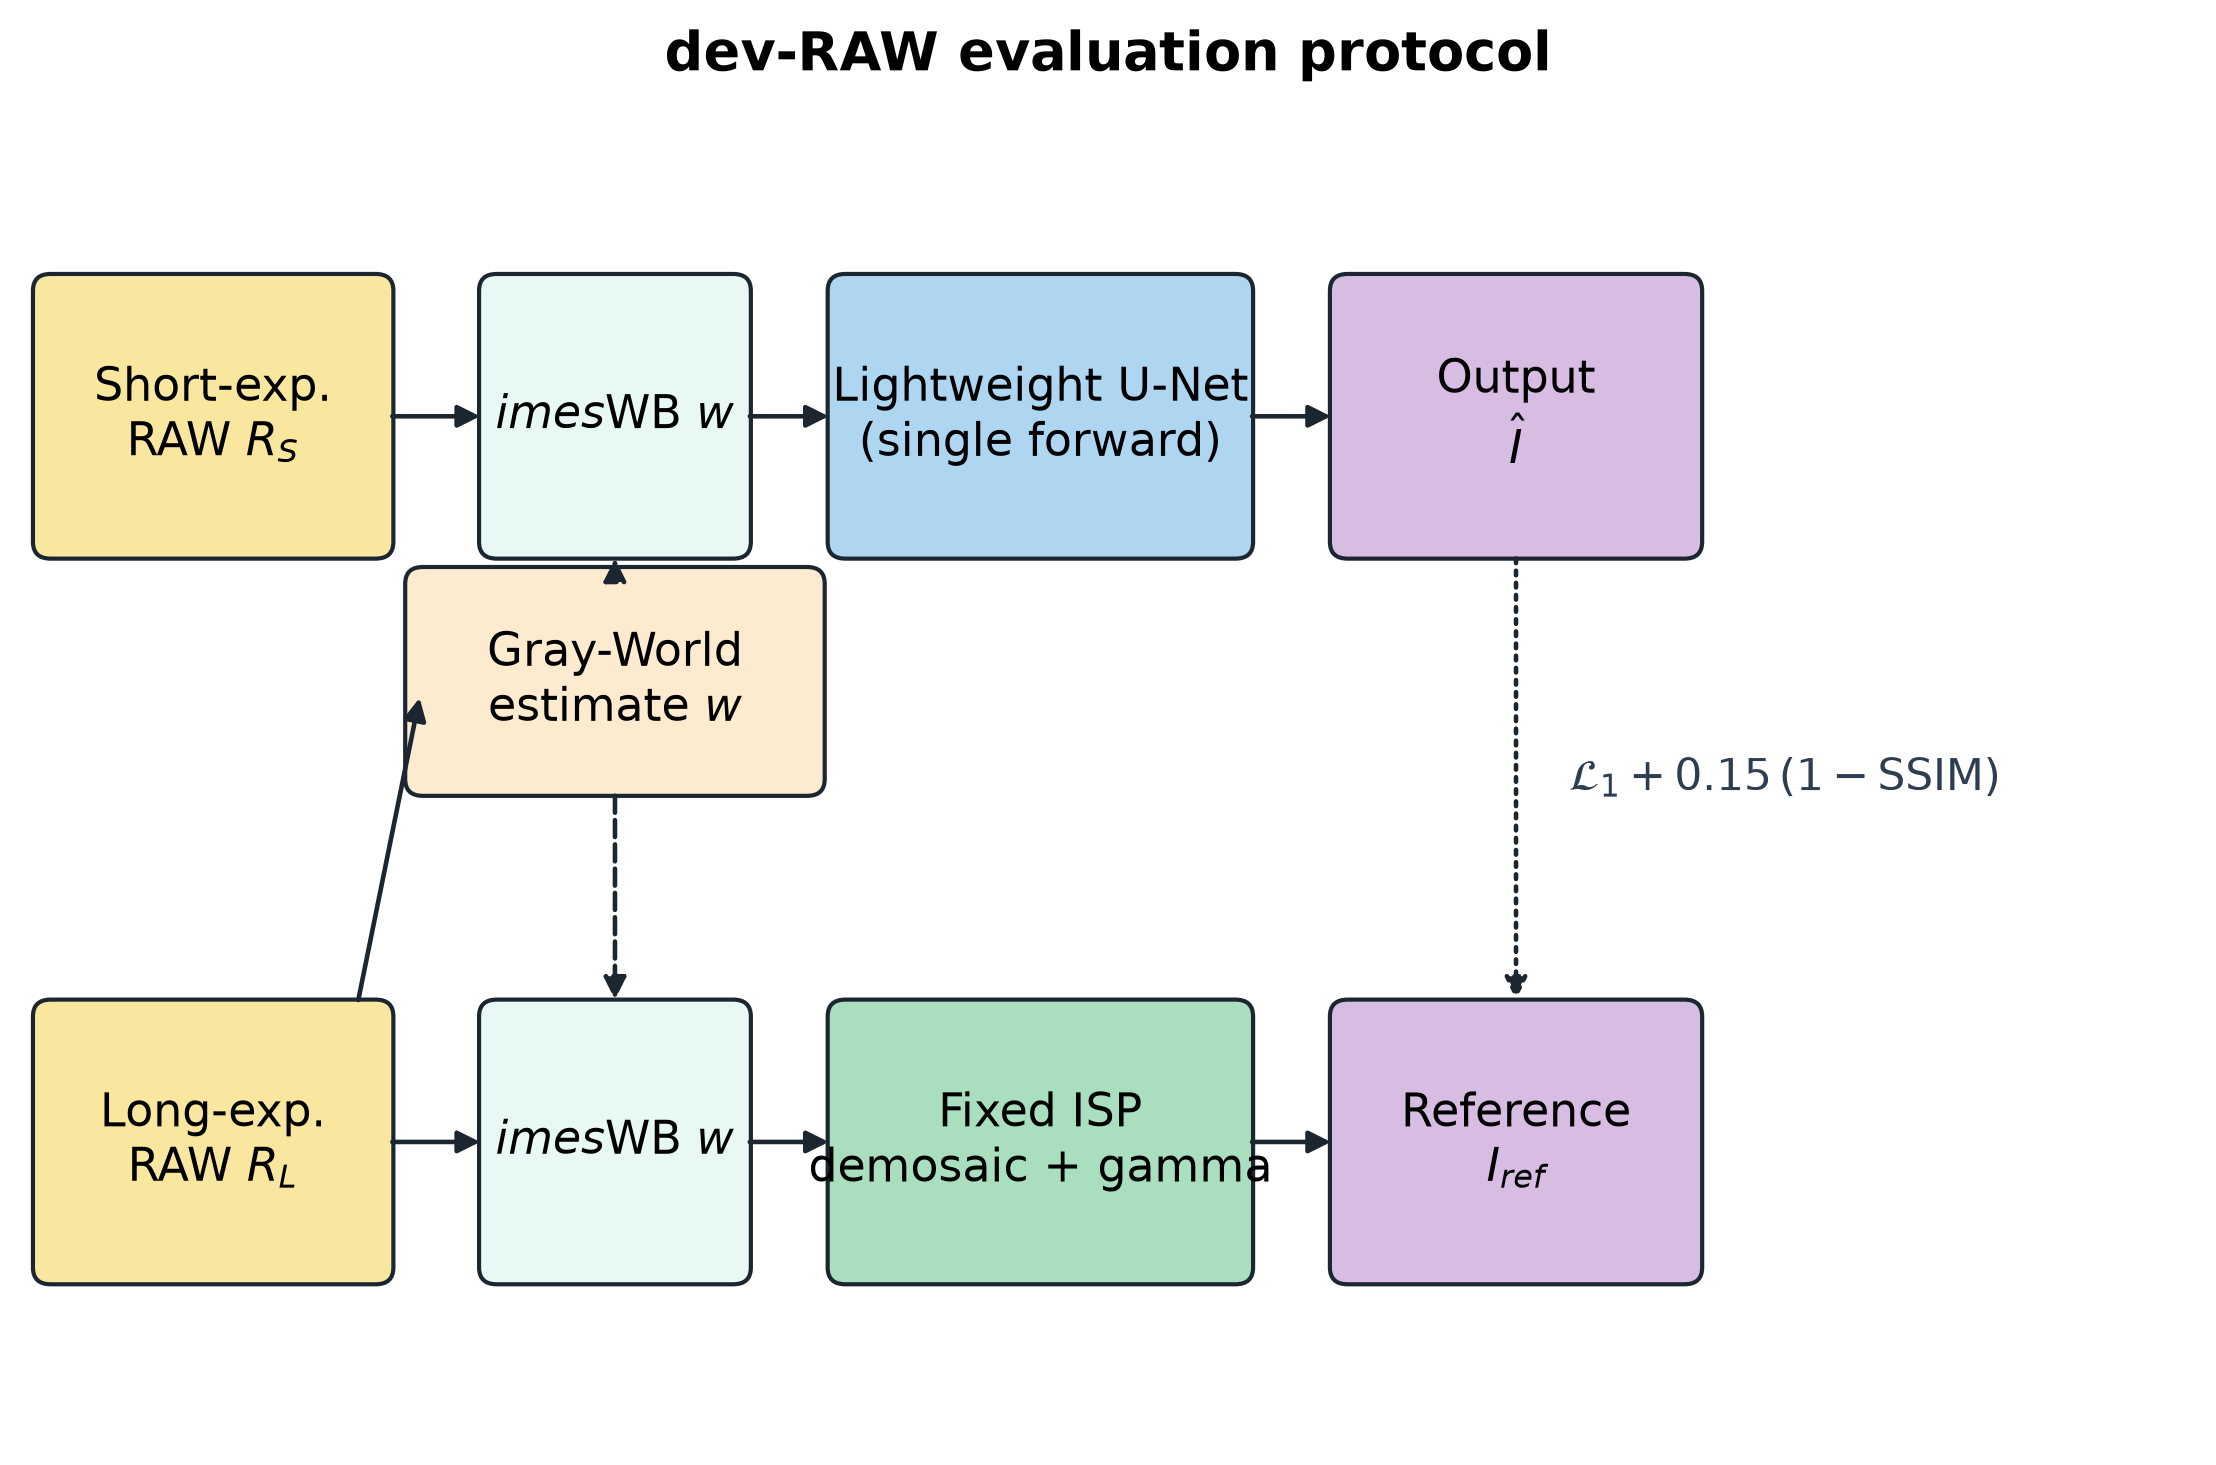
\includegraphics[width=\linewidth]{figures/fig2_protocol.png}
\caption{The dev-RAW evaluation protocol. The short-exposure RAW and the long-exposure RAW share the white-balance coefficients $\mathbf{w}$ estimated from the long-exposure Gray-World assumption; the fixed ISP (white balance $\rightarrow$ demosaic $\rightarrow$ gamma) develops the long-exposure RAW into the reference $I_{ref}$, ensuring the supervision signal and the input reside in the same signal domain.}
\label{fig:protocol}
\end{figure}

\textbf{Problem definition and motivation.} The goal of extremely low-light RAW enhancement is: given a short-exposure RAW signal $R_S$, to recover a clear image of the same scene that would have been captured with a sufficiently long exposure. How the supervision signal (reference) is constructed directly determines the task definition and the numerical evaluation baseline. Using the camera-output JPG directly as the reference introduces a double inconsistency: (1) geometrically, the JPG undergoes lens-distortion correction and cropping, whereas the RAW undergoes about $2\times$ resizing and cropping, so only about 25.8\% of the area can be aligned; (2) in terms of signal, the nonlinear tone mapping of the camera ISP makes the linear RAW signal and the JPG non-differentiably aligned. To avoid these issues, we propose the \textbf{dev-RAW (development-RAW) evaluation protocol}---namely, using ``the image obtained by developing the long-exposure RAW with a fixed ISP'' as the supervisory reference, so that the reference and the input are in the same signal domain.

\textbf{Reference construction.} Let the long-exposure RAW be $R_L$ (after black-level correction, packed Bayer 4-channel linear values). The fixed-ISP development has two steps:
\begin{enumerate}
\item \textbf{Gray-World white balance:} $R_L^{wb} = R_L \cdot \mathbf{w}$, where $\mathbf{w}=[w_R, w_G, w_G, w_B]$ is estimated under the Gray-World assumption (i.e., the average scene reflectance is assumed to be neutral gray).
\item \textbf{Demosaic and gamma:} $I_{ref} = \gamma(\mathrm{demosaic}(R_L^{wb}))$.
\end{enumerate}

\textbf{Input construction.} The short-exposure RAW $R_S$ is processed with the \textbf{same} white-balance coefficients $\mathbf{w}$ (also estimated from the long-exposure RAW) before being fed to the network, ensuring consistency between training and inference.

Under this protocol, the difference between the reference $I_{ref}$ and the input $R_S^{wb}$ arises only from the brightness and noise differences introduced by the different exposure durations. Therefore, the network only needs to learn denoising and brightness recovery, without compensating for ISP differences or geometric registration errors.

\subsection{Network Architecture}
\label{sec:arch}

\begin{figure}[H]
\centering
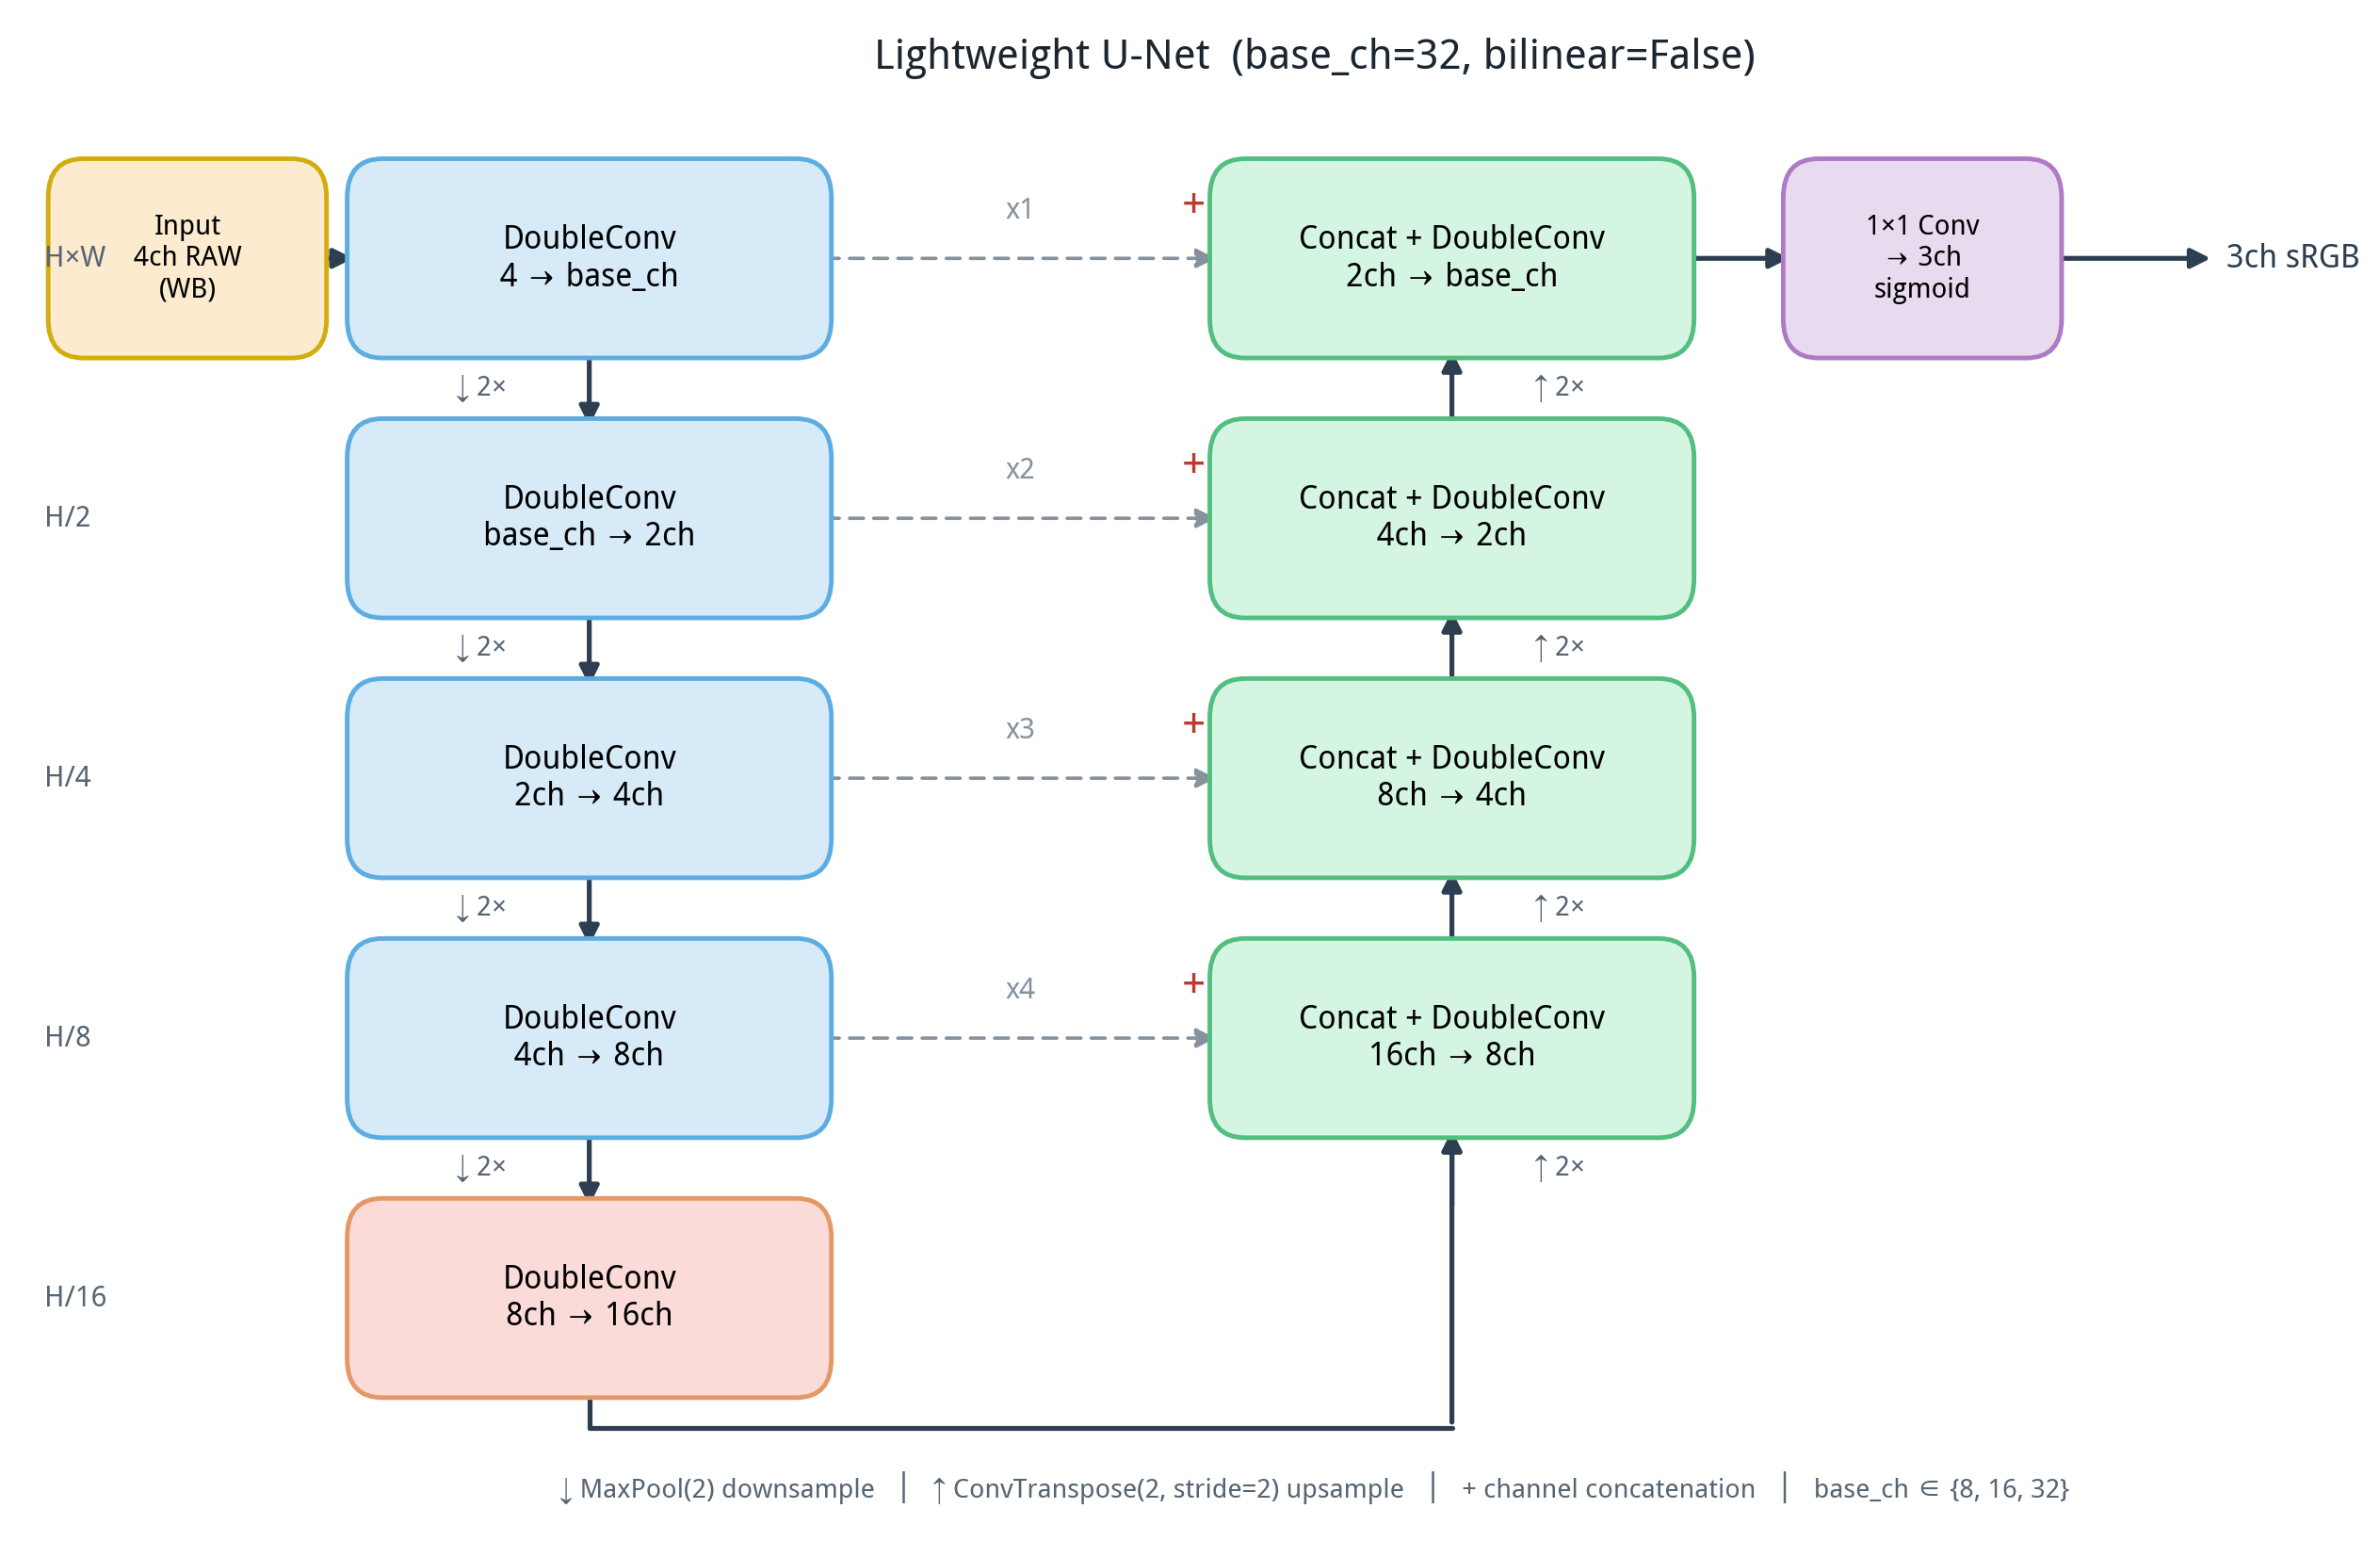
\includegraphics[width=\linewidth]{figures/fig3_architecture.png}
\caption{Overview of the proposed lightweight U-Net. The input is 4-channel packed Bayer (linear values after WB). The encoder downsamples by 4 stages (inc + down1--4, each MaxPool + double convolution) to extract multi-scale features; the bottleneck (down4, $16\times$base\_ch channels) aggregates global information; the decoder upsamples via 4 transposed-convolution stages (up1--4) with skip connections; finally a 1$\times$1 convolution outputs 3-channel RGB followed by sigmoid. base\_ch controls the overall capacity (8/16/32).}
\label{fig:arch}
\end{figure}

\textbf{Design rationale.} Degradation in extremely low-light RAW is dominated by signal-dependent noise: under short exposure, photon shot noise and readout noise are randomly distributed in space, vary in intensity across frequency scales, and fluctuate dramatically with brightness level. The progressively downsampling encoder of U-Net separates noise by scale---shallow layers preserve high-frequency detail while deep layers model low-frequency illumination and global color; skip connections inject high-frequency encoder information directly into the decoder, thereby preserving edges and textures while performing denoising and brightness recovery, and avoiding over-smoothing. The fully convolutional structure does not rely on a fixed input size, performs a single forward pass on arbitrary-resolution RAW, and shares parameters across the whole image, which is naturally suited to deployment scenarios with variable camera RAW sizes and limited resources.

We adopt the classic U-Net encoder--decoder structure (Table~\ref{tab:arch}), with 4-channel packed Bayer (linear values after white balance) as input and 3-channel RGB as output. Downstream of the encoder, a bottleneck aggregates global context, and a symmetric decoder reconstructs the output:

\begin{itemize}
\item \textbf{Encoder:} each stage applies MaxPool2d(2) downsampling and a DoubleConv (two 3$\times$3 convolutions + ReLU), downsampling spatially while widening the channel dimension to build a multi-scale representation.
\item \textbf{Bottleneck:} at the H/16$\times$W/16 resolution, the number of channels is expanded to $16\times$base\_ch to aggregate global context.
\item \textbf{Decoder:} transposed convolutions (ConvTranspose2d, bilinear$=$False) progressively upsample; each stage is concatenated (concat) with the corresponding encoder layer via skip connections and followed by a DoubleConv to progressively restore resolution and detail.
\item \textbf{Output layer:} a 1$\times$1 convolution + sigmoid projects features to 3-channel RGB in [0,1].
\end{itemize}

On this basis, we introduce two lightweight enhancements:

\textbf{SE channel attention.} To enhance feature recalibration at minimal cost, a lightweight SE (Squeeze-and-Excitation) channel attention~\citep{hu2018se} is inserted after each DoubleConv: global average pooling first, then two 1$\times$1 convolutions (reduction$=$16) learn per-channel weights to recalibrate features. This module adds only about 0.06M parameters (7.76M $\rightarrow$ 7.82M at base\_ch$=$32, less than 1\%). Its effectiveness stems from the physical properties of the packed Bayer input: the R, G, and B channels have different sampling rates (G is sampled twice as densely as R/B) and different noise levels, so channel recalibration is equivalent to adaptively adjusting the contribution weight of each color channel in feature space, enabling channel-wise denoising tailored to noise characteristics---this is the underlying reason why SE yields a stable gain (+0.46 dB, see Section~\ref{sec:ablation}) at under 1\% parameter increase.

\textbf{Test-time augmentation (TTA).} At inference, we use 8-fold D4 test-time self-ensemble (horizontal/vertical flips + 90$^\circ$ rotation and their combinations, averaging 8 forward passes), consistent with training augmentation, trading 8 forward passes for a consistent quality gain (see the ablation in Section~\ref{sec:ablation}).

\begin{table}[H]
\centering
\caption{U-Net Architecture (base\_ch$=$32, bilinear$=$False).}
\label{tab:arch}
\begin{tabularx}{\textwidth}{CCCC}
\toprule
Stage & Module & Channels & Resolution \\
\midrule
Input & inc & 4$\rightarrow$32 & H$\times$W \\
Encoder & down1 & 32$\rightarrow$64 & H/2$\times$W/2 \\
Encoder & down2 & 64$\rightarrow$128 & H/4$\times$W/4 \\
Encoder & down3 & 128$\rightarrow$256 & H/8$\times$W/8 \\
Bottleneck & down4 & 256$\rightarrow$512 & H/16$\times$W/16 \\
Decoder & up1 & 512$\rightarrow$256 & H/8$\times$W/8 \\
Decoder & up2 & 256$\rightarrow$128 & H/4$\times$W/4 \\
Decoder & up3 & 128$\rightarrow$64 & H/2$\times$W/2 \\
Decoder & up4 & 64$\rightarrow$32 & H$\times$W \\
Output & outc & 32$\rightarrow$3 & H$\times$W \\
\bottomrule
\end{tabularx}
\end{table}

\textbf{Adjustable capacity.} The hyper-parameter base\_ch controls the base width of channels across layers; base\_ch$=$8/16/32 corresponds to 0.49M/1.94M/7.82M parameters and 82.6/43.3/17.8 FPS (V100). This provides a systematic quality--efficiency trade-off: high-compute platforms can choose base\_ch$=$32 for peak quality, while edge platforms can choose base\_ch$=$8 for real-time processing (see the capacity ablation in Section~\ref{sec:ablation} and Figure~6).

\subsection{Loss Function}

The total loss is defined as a weighted sum of the L1 loss and the structural similarity (SSIM) loss:
\begin{equation}
\mathcal{L} = \mathcal{L}_1 + \lambda_{ssim}\left(1 - \mathrm{SSIM}(\hat{I}, I_{ref})\right)
\end{equation}
where $\mathcal{L}_1 = \|M \odot (\hat{I} - I_{ref})\|_1$ is the masked L1 (computed only over valid pixel regions, $M$ being the valid-region mask), $\hat{I}$ is the network output, and $I_{ref}$ is the dev-RAW reference; $1-\mathrm{SSIM}(\cdot)$ is the structural difference term, and $\lambda_{ssim}=0.15$ is its weight. Chroma-loss and luma-loss variants are also tested in the ablation (see Section~\ref{sec:ablation}).

\textbf{Design rationale.} We choose the L1 loss over the MSE loss because L1 is more robust to pixel-level outliers (noise spikes): in extremely low light, the estimation errors of high-noise pixels follow a heavy-tailed distribution, and the quadratic penalty of MSE would over-amplify the gradients of these pixels, forcing the network to smooth the whole output and lose detail just to suppress a few noisy pixels; the linear penalty of L1 tolerates noise and better preserves detail. The SSIM term compensates for the tendency of L1 to over-average, constraining the structural consistency between the output and the reference in terms of luminance, contrast, and structure. The mask $M$ excludes black borders and invalid pixel regions, preventing the network from learning edge information irrelevant to the task.

\subsection{Dataset}

We use the Sony subset (Sony $\alpha$7RIII) 0.01--0.1~lx level of SIED~\citep{jiang2025sied}, containing 1680 pairs of short-exposure RAW and corresponding long-exposure RAW (Sony 14-bit, black level 512, white level 16383, short-exposure RAW size 1080$\times$1920$\times$4 packed Bayer). Following the official SIED~\citep{jiang2025sied} split, the 1680 scenes are split 1500:180 into train/test sets; the training and test scene IDs are checked one by one to ensure no overlap and avoid data leakage. Note that our evaluation protocol differs from the official SIED~\citep{jiang2025sied} one: the official SIED uses the real-captured normal-light sRGB as the reference and evaluates on the 1500/180-split test set; we instead use the long-exposure RAW developed by a fixed ISP as the supervisory reference (the dev-RAW protocol, see Section~\ref{sec:devraw}), thereby avoiding JPG--RAW misalignment and ISP inconsistency.

To cover the full 0.0001--0.1~lx range of SIED~\citep{jiang2025sied}, we use its Sony subset. SIED realizes the three illuminance ranges in Table~\ref{tab:levels} through laboratory illuminance calibration and calibrated noise injection, yielding 1680 paired samples per level (5040 pairs in total, using the real-captured normal-light sRGB as reference); the synthesis procedure is described in~\citep{jiang2025sied}. A single model jointly covers all three illuminance levels.

\begin{table}[H]
\centering
\caption{Three illuminance levels of SIED.}
\label{tab:levels}
\begin{tabularx}{\textwidth}{CCC}
\toprule
Illuminance range & No. of low-light RAW & Darkness relative to brightest \\
\midrule
0.01--0.1 lux & 1680 & baseline \\
0.001--0.01 lux & 1680 & $\sim$10$\times$ darker \\
0.0001--0.001 lux & 1680 & $\sim$100$\times$ darker \\
\bottomrule
\end{tabularx}
\end{table}

\subsection{Training Setup and Metrics}

The main model is trained on the combined Sony data of the three SIED illuminance levels (0.01--0.1 / 0.001--0.01 / 0.0001--0.001~lx, 5040 training pairs $=$ 1680 scenes $\times$ 3 levels). Training uses PyTorch with batch\_size$=$8, patch\_size$=$512, Adam optimizer (lr$=$2e-4), 100 epochs, on an NVIDIA Tesla V100-SXM2-32GB. Data augmentation includes random flips and rotations.

The evaluation metrics are PSNR$\uparrow$ / SSIM$\uparrow$ / LPIPS(alex)$\downarrow$, with input range [0,1] and LPIPS internally shifted to [-1,1], aligned with the metric convention of SIED~\citep{jiang2025sied}.

Generative AI was not used to generate or analyze the experimental data, results, or figures in this study; all measurements and figures were produced by the authors' own code from real experimental outputs. AI-assisted language tools were used only to polish the English wording and assist with translation; the authors reviewed and edited all output and take full responsibility for the content.

%%%%%%%%%%%%%%%%%%%%%%%%%%%%%%%%%%%%%%%%%%
\section{Results}
\label{sec:results}

\subsection{Main Results}

\begin{figure}[H]
\centering
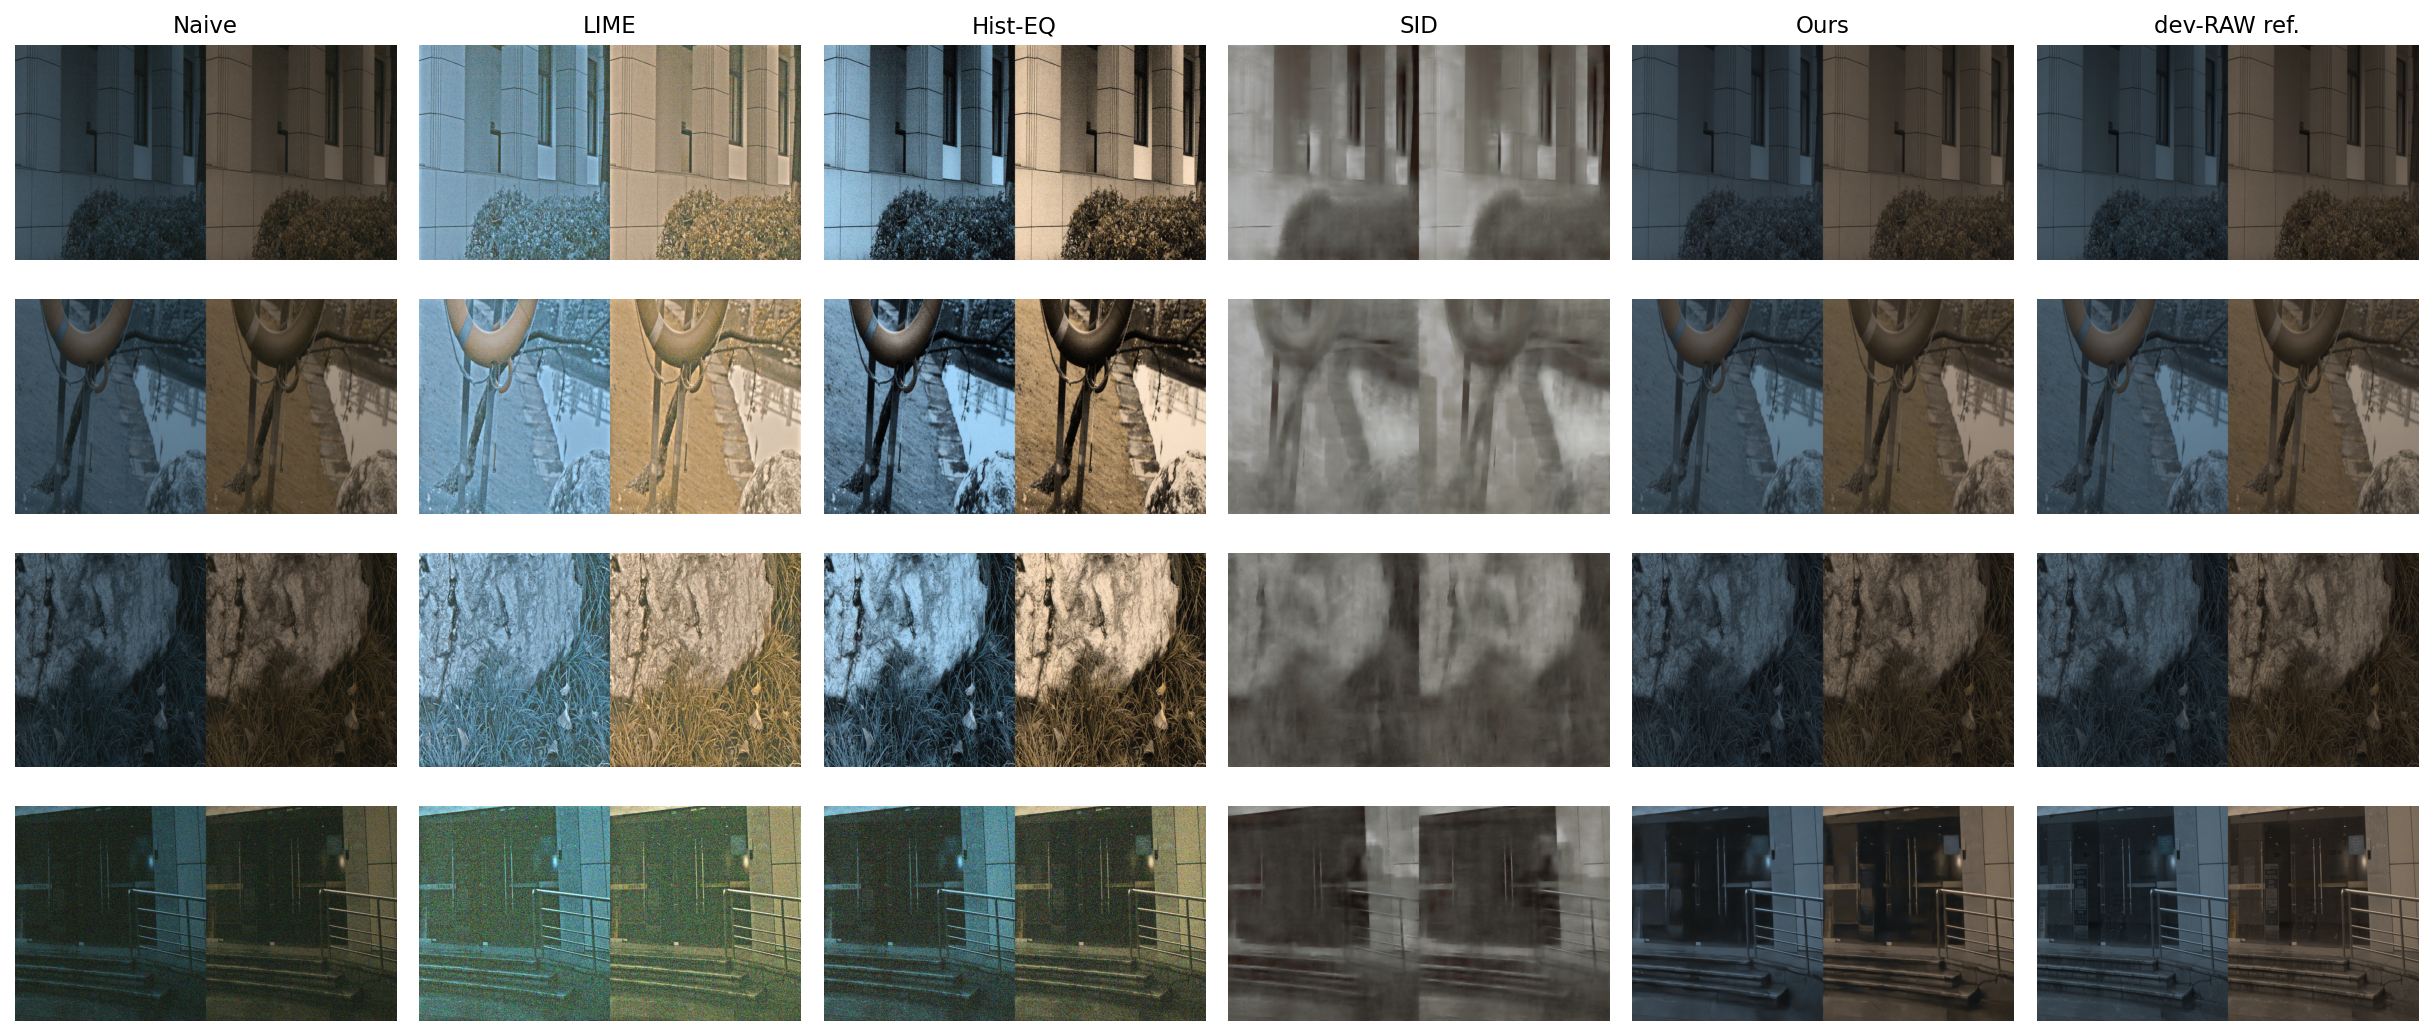
\includegraphics[width=\linewidth]{figures/fig4_visual_compare.png}
\caption{Multi-scene qualitative comparison (four representative frames from the official test set). Each row corresponds to one scene; the columns from left to right are Naive (fixed-ISP amplification baseline), LIME, histogram equalization (Hist-EQ), SID, the proposed method (base\_ch$=$32), and the dev-RAW reference (long-exposure RAW developed by a fixed ISP). Traditional non-learning methods (LIME, Hist-EQ) brighten the scene but introduce strong color casts and noise; the SID baseline shows limited color fidelity and brightness; the proposed method is closest to the reference in noise suppression, brightness recovery, and color fidelity.}
\label{fig:visual}
\end{figure}

\begin{table}[H]
\centering
\caption{Main results on the dev-RAW benchmark (SIED official 180-scene test set, 0.01--0.1~lx, mean$\pm$std).}
\label{tab:main}
\begin{tabularx}{\textwidth}{lCCC}
\toprule
Method & PSNR$\uparrow$ & SSIM$\uparrow$ & LPIPS$\downarrow$ \\
\midrule
LIME~\citep{guo2017lime} (non-learning) & 9.43$\pm$0.80 & 0.1067$\pm$0.1025 & 1.0926$\pm$0.2950 \\
Histogram equalization (non-learning) & 12.35$\pm$2.22 & 0.1293$\pm$0.1167 & 1.0676$\pm$0.3032 \\
Naive (fixed ISP gain) & 21.06$\pm$5.06 & 0.2640$\pm$0.1870 & 0.9122$\pm$0.3324 \\
SID~\citep{chen2018sid} (learning, JPG target) & 16.78$\pm$2.76 & 0.7125$\pm$0.0771 & 0.6320$\pm$0.1169 \\
\textbf{Ours (base\_ch$=$32, multi-illum.+SE)} & \textbf{34.37$\pm$3.29} & \textbf{0.9059$\pm$0.0475} & \textbf{0.1838$\pm$0.1000} \\
\textbf{Ours + 8$\times$ D4 TTA} & \textbf{34.49$\pm$3.29} & \textbf{0.9082$\pm$0.0464} & \textbf{0.1827$\pm$0.1010} \\
\bottomrule
\end{tabularx}
\end{table}

\begin{figure}[H]
\centering
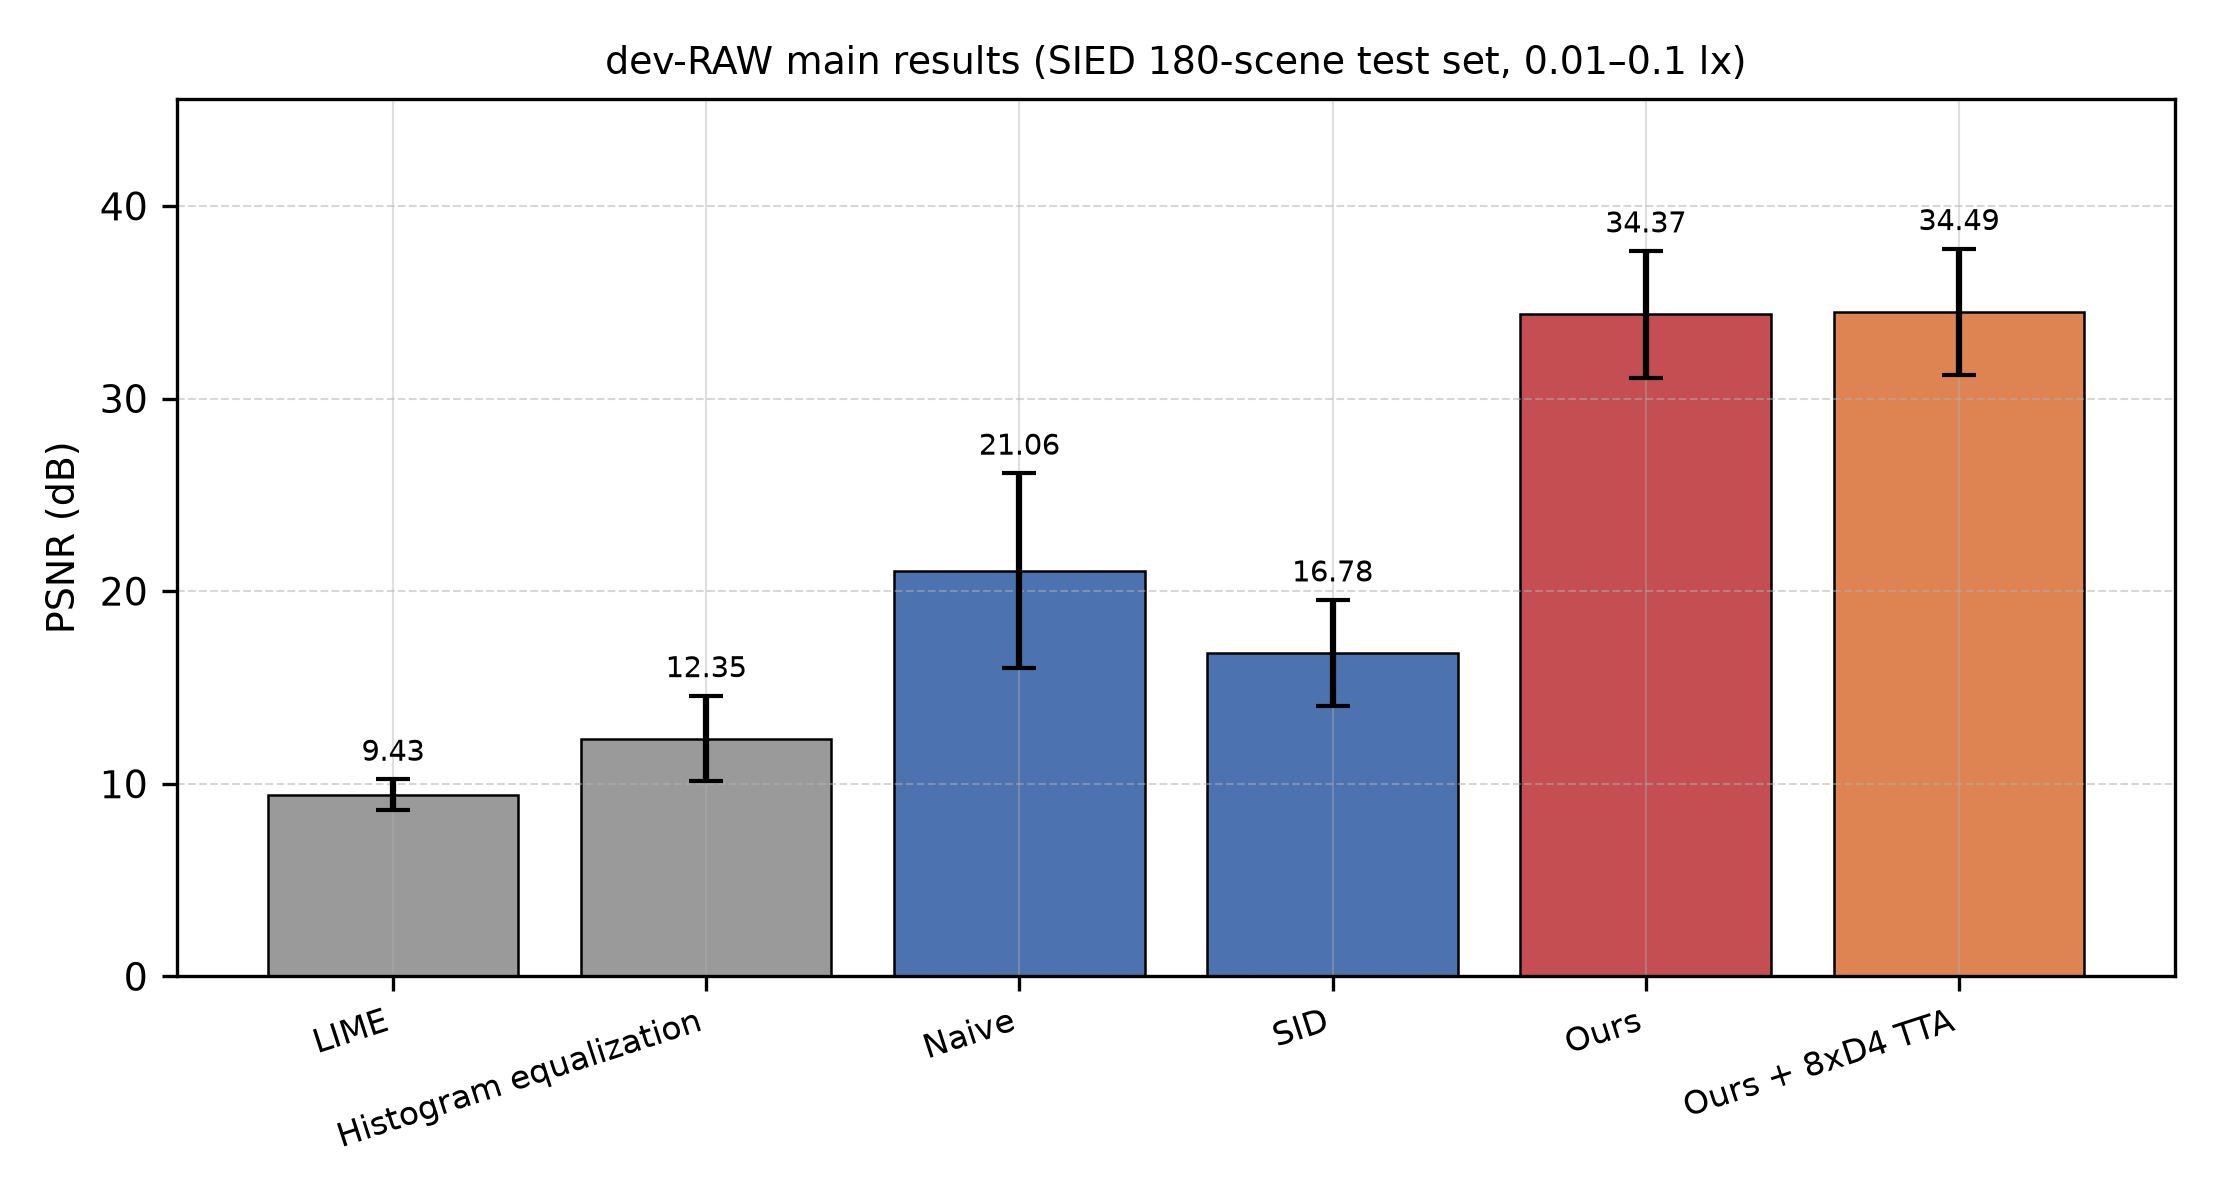
\includegraphics[width=0.8\linewidth]{figures/fig5_psnr_bar.png}
\caption{PSNR bar chart of the main results on the dev-RAW benchmark (SIED official 180-scene test set, 0.01--0.1~lx). Relative to the fixed-ISP amplification baseline (Naive, 21.06~dB), the proposed method (base\_ch$=$32, multi-illuminance $+$ SE) improves PSNR by $+13.31$~dB (34.37~dB), SSIM by $+0.6419$, and LPIPS by $-0.7284$; it also surpasses the sRGB non-learning baselines LIME (9.43~dB) and histogram equalization (12.35~dB) by more than $22$~dB, and the learning-based SID baseline (16.78~dB) by $+17.59$~dB. The 8-fold D4 TTA evaluation adds a further $+0.12$~dB (34.49~dB).}
\label{fig:psnrbar}
\end{figure}

\textbf{Main results.} As summarized in Figure~\ref{fig:psnrbar} and Table~\ref{tab:main}, our method (base\_ch$=$32, multi-illuminance $+$ SE) attains 34.37~dB PSNR / 0.9059 SSIM / 0.1838 LPIPS on the dev-RAW benchmark. Every improvement below is stated relative to an explicit baseline: $+13.31$~dB over the fixed-ISP amplification baseline (Naive, 21.06~dB), which is the primary dev-RAW reference; $+17.59$~dB over the SID-style learning baseline (16.78~dB); $+22.02$~dB over histogram equalization (12.35~dB); and $+24.94$~dB over LIME (9.43~dB). The 8-fold D4 TTA adds a further $+0.12$~dB over the single-forward result, reaching 34.49~dB.

\textbf{Comparison with traditional methods.} As shown in Table~\ref{tab:main}, sRGB-domain traditional non-learning methods are far inferior to ours: LIME~\citep{guo2017lime} refines an illumination map and histogram equalization merely re-distributes intensities; neither models the extreme noise in the RAW domain, and both over-expose by re-brightening images on which the fixed ISP has already applied exposure compensation. Hence their dev-RAW PSNR is only 9.43/12.35~dB, even lower than the naive baseline (21.06~dB). Notably, the SID~\citep{chen2018sid} learning baseline, which uses the same CNN architecture but is trained with aligned JPG as the supervisory target, achieves only 16.78~dB in the dev-RAW domain---its supervision signal and input are in different signal domains (the JPG has undergone the full nonlinear ISP processing), so it cannot effectively guide denoising and brightness recovery in the linear RAW domain, and is therefore far below our dev-RAW-supervised method (34.37~dB). This further demonstrates that extremely low-light RAW enhancement must learn denoising and brightness recovery end-to-end, and the supervisory reference must reside in the same signal domain as the input.

\subsection{Cross-Illuminance Robustness}

We evaluate the single model on each of the three SIED illuminance levels to verify the illuminance generalization of the unified model (Ours, base\_ch$=$32+SE, no TTA), as shown in Table~\ref{tab:crossill}. From 0.01--0.1~lx to 0.0001--0.001~lx (about two orders of magnitude darker), the single-model PSNR drops by only 2.63~dB (34.37 $\rightarrow$ 31.74), verifying the robustness of our method under extreme illuminance. Compared with SIED~\citep{jiang2025sied}, which trains a separate model for each illuminance level, our single-model scheme is more advantageous for deployment efficiency.

\begin{table}[H]
\centering
\caption{Cross-illuminance evaluation (single model, base\_ch$=$32+SE, official 180-scene test set).}
\label{tab:crossill}
\begin{tabularx}{\textwidth}{CCCC}
\toprule
Illuminance (lux) & PSNR$\uparrow$ & SSIM$\uparrow$ & LPIPS$\downarrow$ \\
\midrule
0.01--0.1 & 34.37$\pm$3.29 & 0.9059$\pm$0.0475 & 0.1838$\pm$0.1000 \\
0.001--0.01 & 33.63$\pm$3.80 & 0.8962$\pm$0.0557 & 0.2070$\pm$0.1211 \\
0.0001--0.001 & 31.74$\pm$5.08 & 0.8722$\pm$0.0749 & 0.2640$\pm$0.1690 \\
\bottomrule
\end{tabularx}
\end{table}

\subsection{Cross-Camera Generalization}

To further verify the transfer ability on unseen camera data, we apply the Sony-trained SE model (base\_ch$=$32+SE) \textbf{without any fine-tuning} directly to the SIED Canon subset 0.01--0.1~lx official 180-scene test set (dev-RAW protocol), as shown in Table~\ref{tab:crosscam}. The Sony-trained model achieves 33.05~dB on Canon data without fine-tuning, +10.86~dB over the naive baseline and only 1.32~dB lower than the Sony same-level result (34.37~dB), indicating that the RAW-domain denoising and brightness-recovery knowledge learned by our method generalizes across cameras rather than overfitting to a single sensor's noise characteristics.

\begin{table}[H]
\centering
\caption{Cross-camera generalization (Sony-trained $\rightarrow$ Canon-tested, dev-RAW, 0.01--0.1~lx, mean$\pm$std).}
\label{tab:crosscam}
\begin{tabularx}{\textwidth}{lCCC}
\toprule
Method & PSNR$\uparrow$ & SSIM$\uparrow$ & LPIPS$\downarrow$ \\
\midrule
Naive (fixed ISP gain) & 22.19$\pm$5.72 & 0.3493$\pm$0.2330 & 0.7787$\pm$0.3941 \\
\textbf{Ours (Sony-trained, no fine-tuning)} & \textbf{33.05$\pm$4.01} & \textbf{0.8877$\pm$0.0716} & \textbf{0.2146$\pm$0.1408} \\
\bottomrule
\end{tabularx}
\end{table}

\subsection{Comparison with Published Methods (sRGB Baseline)}

To provide a unified-source efficiency--quality reference, Table~\ref{tab:srgb} lists the published PSNR of representative methods on the SID(Sony) and SIED(Sony, 0.01--0.1~lx) benchmarks (numbers cited from SIED~\citep{jiang2025sied} Table 2/3).

\begin{table}[H]
\centering
\caption{Comparison with published methods (sRGB reference, PSNR$\uparrow$, cited from SIED~\citep{jiang2025sied} Table 2/3).}
\label{tab:srgb}
\begin{tabularx}{\textwidth}{lCCC}
\toprule
Method & Year & SID(Sony) & SIED(Sony, 0.01--0.1~lx) \\
\midrule
SID~\citep{chen2018sid} & 2018 & 28.96 & 21.93 \\
Retinex-RAWMamba~\citep{chen2024rawmamba} & 2024 & 30.62 & 23.94 \\
SIED~\citep{jiang2025sied} (diffusion) & 2025 & 31.20 & 24.98 \\
\bottomrule
\end{tabularx}
\end{table}

\textbf{Evaluation-baseline note.} Our dev-RAW reference (long-exposure RAW developed by a fixed ISP) differs from the sRGB/JPG reference of Table~\ref{tab:srgb}: the former preserves the fixed-ISP mapping in the linear RAW domain, while the latter involves the full nonlinear camera ISP. Therefore our 34.37~dB (dev-RAW) cannot be directly compared with the sRGB numbers in Table~\ref{tab:srgb}. For an honest comparison, on the official SIED sRGB reference (aligned JPG, computed within a mask) we measure the dev-RAW-optimized model at 11.94~dB, while the same-architecture SID-style learning baseline with JPG target scores 13.83~dB---our model is not higher than published methods on the sRGB baseline, which is the expected result of optimizing for the dev-RAW target (linear RAW domain, fixed-ISP development) rather than the sRGB target. Our contribution lies in light weight, single-model multi-illuminance coverage, cross-camera generalization, and efficiency, not in surpassing quality on a unified sRGB baseline.

\subsection{Efficiency Comparison}

Table~\ref{tab:eff} shows that our method far outperforms the diffusion-based SIED in parameters, computation, and speed: the lightest configuration (base\_ch$=$8) has only 0.49M parameters, 82.6~FPS, and a single forward pass, with about two orders of magnitude fewer parameters and over two orders of magnitude faster speed than SIED ($\sim$175M, $<$1~FPS, multi-step denoising). In terms of quality, SIED achieves 24.98/24.51/23.10~dB on SIED(Sony) with heavy computation (Table 2~\citep{jiang2025sied}); our single-forward lightweight network achieves 34.37~dB on the dev-RAW benchmark (SIED Sony 0.01--0.1~lx) (see the evaluation-baseline note above for the convention difference). Together they characterize the two routes of efficiency--quality: ``heavy-computation diffusion vs. lightweight single forward''---this paper provides a systematic trade-off curve for the latter route.

\begin{table}[H]
\centering
\caption{Efficiency comparison (V100, full frame 1080$\times$1920$\times$4 $\rightarrow$ 1080$\times$1920$\times$3).}
\label{tab:eff}
\begin{tabularx}{\textwidth}{lCCCC}
\toprule
Method & Params & MACs & FPS & Forward mode \\
\midrule
Ours (base\_ch$=$8) & 0.49M & 27.6G & 82.6 & Single forward \\
Ours (base\_ch$=$16) & 1.94M & 109.0G & 43.3 & Single forward \\
Ours (base\_ch$=$32, no SE) & 7.76M & 433.3G & 17.8 & Single forward \\
Ours (base\_ch$=$32, +SE) & 7.82M & 433.3G & 17.8 & Single forward \\
SIED~\citep{jiang2025sied} (diffusion) & $\sim$175M$^{*}$ & --- & $<$1 & Multi-step denoising \\
\bottomrule
\end{tabularx}
\vspace{3pt}
{\footnotesize $^{*}$ The exact parameter count of SIED is not verified from public sources; it is marked as approximate for qualitative illustration only.}
\end{table}

\begin{figure}[H]
\centering
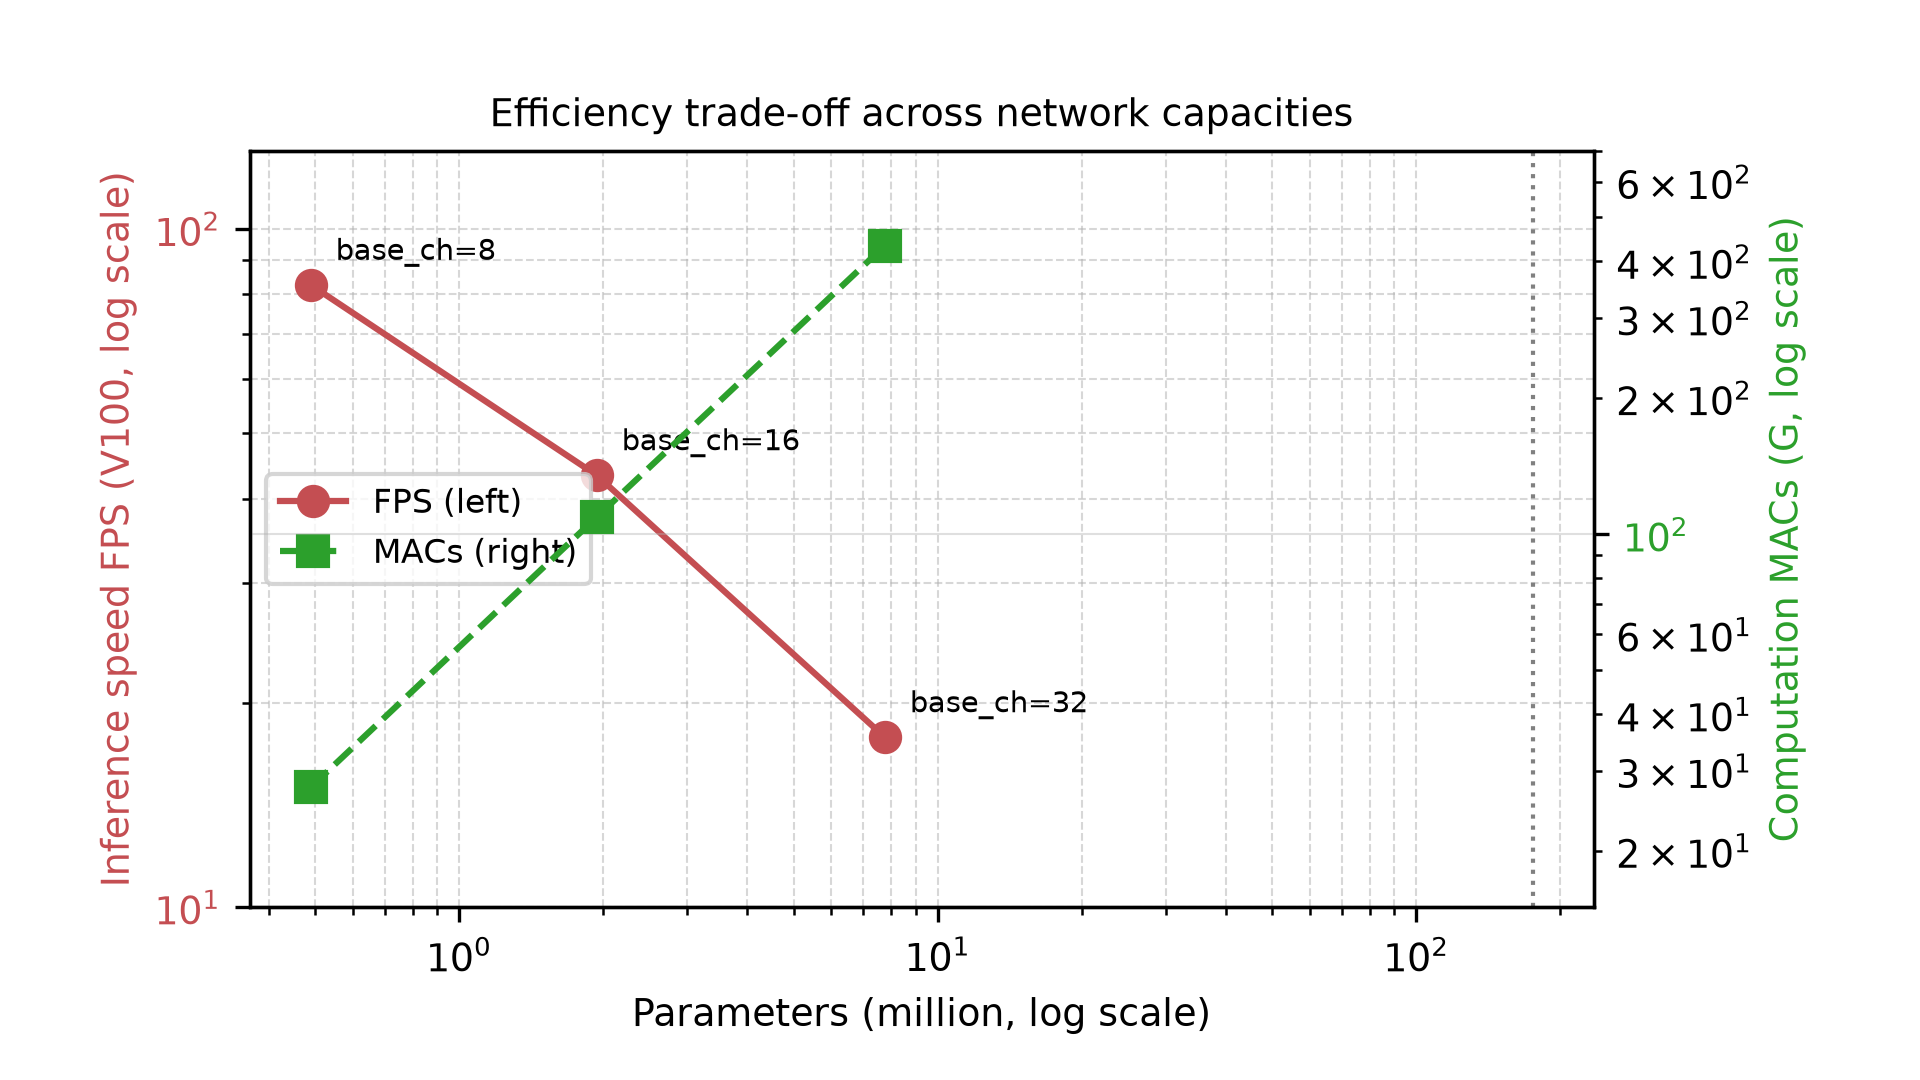
\includegraphics[width=\linewidth]{figures/fig6_efficiency_tradeoff.png}
\caption{Efficiency trade-off curve. The x-axis is the number of parameters (log-log scale). The red curve (left axis) is the inference speed FPS, and the green curve (right axis) is the computation MACs; the three points correspond to base\_ch$=$8/16/32. As the channel count doubles, parameters scale by about 4$\times$, MACs by about 4$\times$, and FPS roughly halves; base\_ch$=$8 (0.49M) has about two orders of magnitude fewer parameters than SIED ($\sim$175M, gray vertical line) and more than 80$\times$ higher FPS. FPS/MACs are measured on the V100; the Jetson edge-device measurements are reported in the ``Edge deployment'' paragraph of Section~\ref{sec:results}.}
\label{fig:tradeoff}
\end{figure}

\textbf{Edge deployment.} To verify real-time performance on resource-constrained platforms, we additionally measure full-frame 1080$\times$1920$\times$4 inference on an NVIDIA Jetson Orin Nano Super edge device (JetPack R36.4.7, 8~GB unified memory, PyTorch 2.3). In fp16, the three tiers base\_ch$=$8/16/32 (0.49M/1.94M/7.76M) reach 7.61/4.78/2.00~FPS, respectively. In fp32, base\_ch$=$8 and base\_ch$=$16 reach 5.98 and 3.27~FPS, while base\_ch$=$32 (7.76M) cannot complete the full-frame forward pass because its fp32 activations exceed the device's available unified memory (fp16 inference proceeds normally). These measurements show that all three capacity tiers can be deployed in fp16 on Jetson-class edge devices, and our lightweight configurations achieve near-real-time enhancement, further validating their practicality and deployability.

\subsection{Ablation Studies}
\label{sec:ablation}

Note: the loss-function ablation (Table~\ref{tab:loss}) and capacity ablation (Table~\ref{tab:cap}) are based on the validation-set PSNR of the single-level 0.01~lx trained model; the SE attention ablation (Table~\ref{tab:se}) and TTA ablation (Table~\ref{tab:tta}) are based on the dev-RAW test results of the three-level jointly trained model on the SIED official 180-scene test set.

\textbf{Loss-function ablation (Table~\ref{tab:loss}).} Fixing base\_ch$=$32, we test four configurations: pure L1, L1+SSIM, L1+chroma loss, and L1+luma loss. L1+SSIM achieves the best validation PSNR and the lowest L1, verifying the contribution of the SSIM term to structural quality; pure chroma/luma regularization brings no additional gain, so the main model adopts L1+SSIM.

\begin{table}[H]
\centering
\caption{Loss-function ablation (base\_ch$=$32, validation set).}
\label{tab:loss}
\begin{tabularx}{\textwidth}{lCC}
\toprule
Loss & Val PSNR$\uparrow$ & Val L1$\downarrow$ \\
\midrule
L1 & 35.43 & 0.01315 \\
L1 + 0.1$\cdot$chroma & 35.38 & 0.01323 \\
L1 + 0.3$\cdot$luma & 35.03 & 0.01391 \\
\textbf{L1 + 0.15$\cdot$SSIM (main)} & \textbf{35.63} & \textbf{0.01294} \\
\bottomrule
\end{tabularx}
\end{table}

\textbf{Capacity ablation (Table~\ref{tab:cap}).} Fixing the L1+0.15$\cdot$SSIM loss, we test the three capacity levels base\_ch$=$8/16/32. Validation PSNR increases with capacity (32 $>$ 16 $>$ 8), which together with the efficiency data reveals the quality--latency trade-off: each doubling of channels increases parameters by about 4$\times$, MACs by about 4$\times$, and roughly halves FPS; users can select a configuration tier according to the target platform's computing power.

\begin{table}[H]
\centering
\caption{Model-capacity ablation (L1+0.15$\cdot$SSIM, validation set).}
\label{tab:cap}
\begin{tabularx}{\textwidth}{CCCCC}
\toprule
base\_ch & Params & MACs & FPS & Val PSNR$\uparrow$ \\
\midrule
8 & 0.49M & 27.6G & 82.6 & 33.95 \\
16 & 1.94M & 109.0G & 43.3 & 35.13 \\
32 & 7.76M & 433.3G & 17.8 & \textbf{35.63} \\
\bottomrule
\end{tabularx}
\end{table}

\textbf{SE channel-attention ablation (Table~\ref{tab:se}).} Fixing base\_ch$=$32, L1+0.15$\cdot$SSIM, and three-level joint training, we compare with and without the SE module. The SE module adds only 0.06M parameters (less than 1\%) and brings a +0.46~dB PSNR improvement, verifying the effectiveness of lightweight channel attention in extremely low-light denoising.

\begin{table}[H]
\centering
\caption{SE channel-attention ablation (base\_ch$=$32, three-level joint training, official 180-scene test set).}
\label{tab:se}
\begin{tabularx}{\textwidth}{lCCCC}
\toprule
Config & Params & PSNR$\uparrow$ & SSIM$\uparrow$ & LPIPS$\downarrow$ \\
\midrule
w/o SE & 7.76M & 33.91$\pm$3.62 & 0.9050$\pm$0.0483 & 0.1831$\pm$0.1005 \\
\textbf{+SE (main)} & \textbf{7.82M} & \textbf{34.37$\pm$3.29} & \textbf{0.9059$\pm$0.0475} & \textbf{0.1838$\pm$0.1000} \\
\bottomrule
\end{tabularx}
\end{table}

\textbf{TTA ablation (Table~\ref{tab:tta}).} On the main model (base\_ch$=$32+SE), we compare a single forward pass with 8-fold D4 TTA. 8-fold D4 TTA brings +0.12~dB PSNR and +0.0023 SSIM gains, while LPIPS also slightly decreases (-0.0011); all three metrics improve consistently, indicating that the transformation set consistent with training augmentation effectively reduces inference variance. On the configuration without SE, the TTA gain is +0.17~dB (33.91 $\rightarrow$ 34.08), showing that TTA is effective for both SE and non-SE models.

\begin{table}[H]
\centering
\caption{TTA ablation (base\_ch$=$32+SE, official 180-scene test set).}
\label{tab:tta}
\begin{tabularx}{\textwidth}{lCCCC}
\toprule
Config & Forward passes & PSNR$\uparrow$ & SSIM$\uparrow$ & LPIPS$\downarrow$ \\
\midrule
Single forward & 1 & 34.37$\pm$3.29 & 0.9059$\pm$0.0475 & 0.1838$\pm$0.1000 \\
\textbf{8$\times$ D4 TTA} & 8 & \textbf{34.49$\pm$3.29} & \textbf{0.9082$\pm$0.0464} & \textbf{0.1827$\pm$0.1010} \\
\bottomrule
\end{tabularx}
\end{table}

%%%%%%%%%%%%%%%%%%%%%%%%%%%%%%%%%%%%%%%%%%
\section{Discussion}
\label{sec:discussion}

The results demonstrate that a lightweight fully-convolutional U-Net can deliver usable restoration quality for extremely low-light RAW enhancement at a fraction of the computational cost of diffusion-based or Transformer-based methods. The dev-RAW protocol plays a key role: by ensuring the reference and input reside in the same signal domain, the network is freed from compensating for ISP differences or geometric misalignment, allowing it to focus on the core tasks of denoising and brightness recovery. This is evidenced by the large gap (34.37 vs. 16.78~dB) between our dev-RAW-supervised model and the same-architecture JPG-supervised SID baseline.

The single-model multi-illuminance design is another important factor. Unlike SIED, which trains a separate model per illuminance level, our model jointly covers all three SIED levels and still maintains graceful degradation (only 2.63~dB drop from the brightest to the darkest level). This makes deployment simpler and more efficient. The cross-camera experiment (33.05~dB on Canon without fine-tuning) further suggests that the learned knowledge is not overfitted to a single sensor's noise characteristics.

The efficiency--quality trade-off is the central theme. With base\_ch$=$8 (0.49M parameters, 82.6~FPS), our method provides a real-time solution for resource-constrained platforms, while base\_ch$=$32 (7.82M, 17.8~FPS) offers higher quality. The SE channel attention and D4 TTA provide consistent, low-cost quality gains (+0.46~dB and +0.12~dB, respectively).

We openly acknowledge the limitation that our method is not directly comparable to sRGB-baseline methods in terms of PSNR, because the dev-RAW reference differs from the sRGB/JPG reference. The contribution of this work is therefore positioned in efficiency, lightweight design, single-model multi-illuminance coverage, and cross-camera generalization, rather than in surpassing state-of-the-art quality on a unified sRGB benchmark.

%%%%%%%%%%%%%%%%%%%%%%%%%%%%%%%%%%%%%%%%%%
\section{Conclusions}
\label{sec:conclusion}

This paper proposes a lightweight fully-convolutional U-Net for extremely low-light RAW image enhancement, adopting the dev-RAW evaluation protocol that uses a long-exposure RAW developed by a fixed ISP as the reference to avoid JPG--RAW misalignment and ISP inconsistency. Unlike SIED~\citep{jiang2025sied}, which trains a separate model for each illuminance level, we use a \textbf{single model to uniformly cover the three SIED illuminance levels of 0.01--0.1 / 0.001--0.01 / 0.0001--0.001~lx} (5040 paired synthetic samples) without any illuminance prior. On the SIED official 180-scene test set (0.01~lx, dev-RAW), the base\_ch$=$32+SE configuration achieves 34.37~dB PSNR, 13.31~dB higher than the fixed-ISP amplification baseline and significantly better than the same-architecture SID-style learning baseline with JPG target (16.78~dB); 8-fold D4 TTA further improves it to 34.49~dB. The single model's PSNR drops gracefully by only 2.63~dB across illuminance levels (34.37 $\rightarrow$ 31.74), and it reaches 33.05~dB on the Canon camera without fine-tuning. Ablation studies verify: the L1+SSIM loss is optimal, increasing capacity brings quality gains, the SE channel attention brings +0.46~dB with less than 1\% parameter overhead, and TTA brings +0.12~dB. The lightest base\_ch$=$8 configuration has only 0.49M parameters at 82.6~FPS, providing an efficient real-time solution for extremely low-light RAW enhancement. We honestly state that the dev-RAW baseline and the sRGB baseline are not directly comparable, and position this work as efficiency-oriented. Future work will explore fair comparisons with diffusion methods under a unified sRGB baseline, and extend the dev-RAW protocol to a broader range of sensors and scenarios.

%%%%%%%%%%%%%%%%%%%%%%%%%%%%%%%%%%%%%%%%%%
\authorcontributions{Conceptualization, X.Z. and S.Y.; methodology, X.Z.; software, X.Z.; validation, X.Z. and S.Y.; formal analysis, X.Z.; investigation, X.Z.; data curation, X.Z.; writing---original draft preparation, X.Z.; writing---review and editing, X.Z. and S.Y.; visualization, X.Z.; supervision, S.Y.; project administration, S.Y. All authors have read and agreed to the published version of the manuscript.}

\funding{This research received no external funding.}

\institutionalreview{Not applicable.}

\informedconsent{Not applicable.}

\dataavailability{The image data used in this study is the publicly available SIED (See-in-the-Extremely-Dark) dataset, available at https://github.com/JianghaiSCU/SIED. The code and trained models generated during this study are available from the corresponding author upon reasonable request.}

\acknowledgments{During the preparation of this manuscript, the author(s) used AI-assisted tools for language polishing and translation. The authors have reviewed and edited the output and take full responsibility for the content of this publication. The authors also thank the SIED dataset authors for making their data publicly available.}

\conflictsofinterest{The authors declare no conflicts of interest.}

%%%%%%%%%%%%%%%%%%%%%%%%%%%%%%%%%%%%%%%%%%
\abbreviations{Abbreviations}{%
The following abbreviations are used in this manuscript:\\

\noindent 
\begin{tabular}{@{}ll}
RAW & Raw image sensor data (Bayer) \\
ISP & Image Signal Processor \\
SNR & Signal-to-Noise Ratio \\
PSNR & Peak Signal-to-Noise Ratio \\
SSIM & Structural Similarity Index \\
LPIPS & Learned Perceptual Image Patch Similarity \\
SE & Squeeze-and-Excitation \\
TTA & Test-Time Augmentation \\
U-Net & U-shaped Network \\
FPS & Frames Per Second \\
MACs & Multiply-Accumulate Operations
\end{tabular}
}

%%%%%%%%%%%%%%%%%%%%%%%%%%%%%%%%%%%%%%%%%%
\reftitle{References}

\begin{thebibliography}{999}

\bibitem{chen2018sid}
Chen, C.; Chen, Q.; Xu, J.; Koltun, V. Learning to See in the Dark. In \emph{Proceedings of the IEEE Conference on Computer Vision and Pattern Recognition (CVPR)}, Salt Lake City, UT, USA, 18--23 June 2018; pp. 3291--3300.

\bibitem{guo2017lime}
Guo, X.; Li, Y.; Ling, H. LIME: Low-Light Image Enhancement via Illumination Map Estimation. \emph{IEEE Trans. Image Process.} {\bf 2017}, \emph{26}, 982--993.

\bibitem{wei2018retinexnet}
Wei, C.; Wang, W.; Yang, W.; Liu, J. Deep Retinex Decomposition for Low-Light Enhancement. In \emph{Proceedings of the British Machine Vision Conference (BMVC)}, Newcastle, UK, 3--6 September 2018.

\bibitem{jiang2025sied}
Jiang, H.; Guan, B.; Liu, Z.; Liu, X.; Yu, J.; Liu, Z.; Han, S.; Liu, S. Learning to See in the Extremely Dark. In \emph{Proceedings of the IEEE/CVF International Conference on Computer Vision (ICCV)}, 2025; pp. 7676--7685.

\bibitem{cai2023retinexformer}
Cai, Y.; Bian, H.; Lin, J.; Wang, H.; Timofte, R.; Zhang, Y. Retinexformer: One-Stage Retinex-Based Transformer for Low-Light Image Enhancement. In \emph{Proceedings of the IEEE/CVF International Conference on Computer Vision (ICCV)}, Paris, France, 2--6 October 2023; pp. 12504--12513.

\bibitem{wang2022llflow}
Wang, Y.; Wan, R.; Yang, W.; Li, H.; Chau, L.-P.; Kot, A.C. LLFlow: Low-Light Image Enhancement with Normalizing Flow. In \emph{Proceedings of the AAAI Conference on Artificial Intelligence}, 2022; Vol. 36, pp. 2604--2612.

\bibitem{zamir2022restormer}
Zamir, S.W.; Arora, A.; Khan, S.; Hayat, M.; Khan, F.S.; Yang, M.-H. Restormer: Efficient Transformer for High-Resolution Image Restoration. In \emph{Proceedings of the IEEE/CVF Conference on Computer Vision and Pattern Recognition (CVPR)}, New Orleans, LA, USA, 18--24 June 2022; pp. 5718--5729.

\bibitem{chen2024rawmamba}
Chen, X.; Huang, P.; Feng, X.; Zhang, D.; Han, L.; Han, J. Retinex-RAWMamba: Bridging Demosaicing and Denoising for Low-Light RAW Image Enhancement. \emph{arXiv} {\bf 2024}, arXiv:2409.07040.

\bibitem{jiang2023difll}
Jiang, H.; Luo, A.; Han, S.; Fan, H.; Liu, S. Low-Light Image Enhancement with Wavelet-Based Diffusion Models. \emph{ACM Trans. Graph.} {\bf 2023}, \emph{42}, 238.

\bibitem{jiang2024lightendiffusion}
Jiang, H.; Luo, A.; Liu, X.; Han, S.; Liu, S. LightenDiffusion: Unsupervised Low-Light Image Enhancement with Latent-Retinex Diffusion Models. In \emph{Proceedings of the European Conference on Computer Vision (ECCV)}, 2024; pp. 161--179.

\bibitem{wen2023ldmisp}
Wen, Q.; Rao, Z.; Xing, Y.; Chen, Q. LDM-ISP: Enhancing Neural ISP for Low Light with Latent Diffusion Models. \emph{arXiv} {\bf 2023}, arXiv:2312.01027.

\bibitem{liao2025gmmoe}
Liao, M.; Dong, H.B.; Wang, X.; Ubul, K.; Shao, Y.; Yan, Z. GM-MoE: Low-Light Enhancement with Gated-Mechanism Mixture-of-Experts. In \emph{Proceedings of the IEEE/CVF International Conference on Computer Vision (ICCV)}, 2025.

\bibitem{chen2025hima}
Chen, X.; Huang, P.; Han, L.; Zhang, D.; Han, J. Rethinking Efficient Hierarchical Mixing Architecture for Low-Light RAW Image Enhancement. \emph{arXiv} {\bf 2025}, arXiv:2510.15497.

\bibitem{feijoo2025darkir}
Feijoo, D.; Benito, J.C.; Garcia, A.; Conde, M.V. DarkIR: Robust Low-Light Image Restoration. In \emph{Proceedings of the IEEE/CVF Conference on Computer Vision and Pattern Recognition (CVPR)}, 2025.

\bibitem{benito2025flol}
Benito, J.C.; Feijoo, D.; Garcia, A.; Conde, M.V. FLOL: Fast Baselines for Real-World Low-Light Enhancement. \emph{arXiv} {\bf 2025}, arXiv:2501.09718.

\bibitem{kong2025lasq}
Kong, D.; Yang, Z.; Li, S.; Zhi, S.; Liu, L.; Liu, Z.; Xia, J. Luminance-Aware Statistical Quantization: Unsupervised Hierarchical Learning for Illumination Enhancement. \emph{arXiv} {\bf 2025}, arXiv:2511.01510.

\bibitem{zhang2019kind}
Zhang, Y.; Zhang, J.; Guo, X. Kindling the Darkness: A Practical Low-Light Image Enhancer. In \emph{Proceedings of the ACM Multimedia Conference (ACM MM)}, Nice, France, 21--25 October 2019.

\bibitem{guo2020zerodce}
Guo, C.; Li, C.; Guo, J.; Loy, C.C.; Hou, J.; Kwong, S.; Cong, R. Zero-Reference Deep Curve Estimation for Low-Light Image Enhancement. In \emph{Proceedings of the IEEE/CVF Conference on Computer Vision and Pattern Recognition (CVPR)}, Seattle, WA, USA, 13--19 June 2020; pp. 1780--1789.

\bibitem{zamir2020cycleisp}
Zamir, S.W.; Arora, A.; Khan, S.; Hayat, M.; Khan, F.S.; Yang, M.-H.; Shao, L. CycleISP: Real Image Restoration via Improved Data Synthesis. In \emph{Proceedings of the IEEE/CVF Conference on Computer Vision and Pattern Recognition (CVPR)}, Seattle, WA, USA, 13--19 June 2020; pp. 2693--2702.

\bibitem{xia2023diffir}
Xia, B.; Zhang, Y.; Wang, S.; Wang, Y.; Wu, X.; Tian, Y.; Yang, W.; Van Gool, L. DiffIR: Efficient Diffusion Model for Image Restoration. In \emph{Proceedings of the IEEE/CVF International Conference on Computer Vision (ICCV)}, Paris, France, 2--6 October 2023.

\bibitem{hu2018se}
Hu, J.; Shen, L.; Sun, G. Squeeze-and-Excitation Networks. In \emph{Proceedings of the IEEE Conference on Computer Vision and Pattern Recognition (CVPR)}, Salt Lake City, UT, USA, 18--23 June 2018; pp. 7132--7141.

\bibitem{wu2022uretex}
Wu, W.; Weng, J.; Zhang, P.; Wang, X.; Yang, W.; Jiang, J. URetinex-Net: Retinex-Based Deep Unfolding Network for Low-Light Image Enhancement. In \emph{Proceedings of the IEEE/CVF Conference on Computer Vision and Pattern Recognition (CVPR)}, New Orleans, LA, USA, 18--24 June 2022; pp. 5901--5910.

\bibitem{wang2023llformer}
Wang, T.; Zhang, K.; Shen, T.; Luo, W.; Stenger, B.; Lu, T. Ultra-High-Definition Low-Light Image Enhancement: A Benchmark and Transformer-Based Method. In \emph{Proceedings of the AAAI Conference on Artificial Intelligence}, 2023; Vol. 37, pp. 2654--2662.

\bibitem{hou2023gsad}
Hou, J.; Zhu, Z.; Hou, J.; Liu, H.; Zeng, H.; Yuan, H. Global Structure-Aware Diffusion Process for Low-Light Image Enhancement. In \emph{Advances in Neural Information Processing Systems (NeurIPS)}, 2023.

\bibitem{yi2023diffretinex}
Yi, X.; Xu, H.; Zhang, H.; Tang, L.; Ma, J. Diff-Retinex: Rethinking Low-Light Image Enhancement with a Generative Diffusion Model. In \emph{Proceedings of the IEEE/CVF International Conference on Computer Vision (ICCV)}, Paris, France, 2--6 October 2023; pp. 12302--12311.

\bibitem{xu2022snraware}
Xu, X.; Wang, R.; Fu, C.-W.; Jia, J. SNR-Aware Low-Light Image Enhancement. In \emph{Proceedings of the IEEE/CVF Conference on Computer Vision and Pattern Recognition (CVPR)}, New Orleans, LA, USA, 18--24 June 2022; pp. 17714--17724.

\bibitem{chen2019smid}
Chen, C.; Chen, Q.; Do, M.N.; Koltun, V. Seeing Motion in the Dark. In \emph{Proceedings of the IEEE/CVF International Conference on Computer Vision (ICCV)}, Seoul, Republic of Korea, 27 October--2 November 2019; pp. 3185--3194.

\bibitem{ignatov2020pynet}
Ignatov, A.; Van Gool, L.; Timofte, R. Replacing Mobile Camera ISP with a Single Deep Learning Model. In \emph{Proceedings of the IEEE/CVF Conference on Computer Vision and Pattern Recognition Workshops (CVPRW)}, Seattle, WA, USA, 14--19 June 2020; pp. 2275--2285.

\bibitem{zamir2020mirnet}
Zamir, S.W.; Arora, A.; Khan, S.; Hayat, M.; Khan, F.S.; Yang, M.-H.; Shao, L. Learning Enriched Features for Real Image Restoration and Enhancement. In \emph{Proceedings of the European Conference on Computer Vision (ECCV)}, Glasgow, UK, 23--28 August 2020; pp. 492--511.

\bibitem{guo2024mambair}
Guo, H.; Li, J.; Dai, T.; Ouyang, Z.; Ren, X.; Xia, S.-T. MambaIR: A Simple Baseline for Image Restoration with State-Space Model. In \emph{Proceedings of the European Conference on Computer Vision (ECCV)}, 2024; pp. 222--241.

\end{thebibliography}

\PublishersNote{}
\end{document}
